\chapter{Technická analýza}
\label{chap:TechnicalAnalysis}
Dělat informovaná rozhodnutí je podstata každého obchodníka. V akciových trzích se významně používá fundamentální analýza používaná pro budoucí odhad
chování trendu trhu. Fundament se zabývá vnitřní hodnotou trhu, která je spjatá s obchodními výsledky podniků obchodovaných na burze. Tyto dvě faktory,
tedy dlouhodobé obchodní výsledky podniků často korelují právě s hodnotou akcií. Vnitřní hodnota trhu je pak odhadována za momentální hodnotou jmění
těchto firem. Odhady lze dělat z veřejně dostupných dat, například ze zveřejněných účetních uzávěrek, vyplacených dividend, nových produktů nebo různých ekonomických zpráv.
Oproti tomu, technická analýza \cite{analysis:first-steps}\cite{analysis:cambridge} se snaží odhadnout budoucí pohyb tržních cen aktiv (forex, akcie, kryptoměny) na základě dostupných historických dat, převážně
z ceny a objemu minulých uzavřených obchodů. Tato kapitola se podrobněji věnuje technické analýze, její historií, z čeho technická analýza vychází.
Zaobírá se několika metodami používanými při této metodě předpovědi vývoje trhu.


\section{Historie}
První náznaky principů technické analýzy se začaly objevovat už v 17. století v práci Josepha de la Vegy o holandských trzích. O století později začíná
rozvoj dalších metody v Asii, která se postupně vyvíjí v použití svíčkové technicky. Dnes se jedná o nejpoužívanější nástroj pro vytváření finančních grafů.
V první půlce 20. století vznikají první knihy zaměřené na technickou analýzu trhu. V té době se jedná převážně o techniky zaměřené na analýzy trendu a
grafové vzory, jelikož výpočetní síla počítačů pro statistickou analýzu nebyla dostupná. Některé z těchto knih, převážně práce Roberta D. Edwardse a Johna
Mageeho \emph{Technical Analysis of Stock Trends}, se považují za klíčové v tomto oboru a zůstávají platné dodnes. V posledních dekádách bylo vytvořeno
mnoho dalších technických nástrojů a teorií, čím dál více využívající výpočetní algoritmy a postupy podpořené počítači.


\section{Principy}
Techničtí analytici věří ve 3 hlavní principy. První z nich zní takto: \emph{Ceny se pohybují v trendech}. Tedy, že tržní cena buďto roste, klesá, nebo se pohybuje
pouze do strany, též označováno jako stagnace. Druhý z těchto principů je: \emph{Historie má tendenci se opakovat}. Pokud se historie
opakuje, musí v grafech, které vizualizují vývoj trhu, existovat jisté vzory předpovídající nastávající trend. Posledním principem je tvrzení, že \emph{tržní očekávání
    je reflektováno a započteno na hodnotě aktiva}. Pokud existují novinky, předpovídající, nebo naznačující vzestup například zemědělského trhu díky úrodné sezóně, je toto
očekávání již pozitivně reflektováno na hodnotě akcií zemědělských firem a lze to tím pádem vyčíst i z grafů. Jelikož vzory hrají velkou roli v oboru technické analýzy
je následují sekce zaměřená na popis, identifikaci a význam několika vzorů.


\section{Grafové vzory}
\label{sec:ChartPatterns}
Grafové vzory \cite{chart:patterns} jsou opakovaně formující se útvary. V technické analýze jsou využívané jako signály buďto přetrvávání nebo obratu momentálního trendu. Vzory se formují při vykreslení
tržních cen na grafu. Typickým a nejčastěji používaným grafem, je graf svíčkový, vyobrazený na obrázku \ref{subfig:candlestickchart}.
Vzory lze pak
pozorovat na posloupnosti několika po sobě jdoucích svíček. Důležitým faktorem při rozpoznávání vzorů je zobrazené časové rozpětí, které investor pozoruje. Ne vždy mohou
být vzory dobře rozpoznatelné lidským okem. Významnost vzoru časem klesá. Čím později je detekován, tím je méně použitelný.
Existují pokusy \cite{pattern-recognition-using-decision-trees} použít strojové učení pro detekci těchto vzorů, jako například práce
autorů \emph{Marc Velay a Fabrice Daniel} \cite{pattern-recognition-using-ai}, kterým
se podařilo dosáhnout 97\% recallu\footnote{Recall je metrika, která kvantifikuje počet vybraných správných výsledků ze všech možných správných výsledků.}, ale model uměl detekovat pouze 1 vzor.


\subsection{Head and shoulders}
První a zároveň z jeden více známých obratových vzorů je \enquote{Head and shoulders} (Hlava a ramena), viditelný na obrázku \ref{fig:head-n-shoulders}. Jak název napovídá, formace svíček tvoří podobu ramen a hlavy způsobenou
3 kopci a 2 dolinami z čehož je prostřední kopec vyšší než zbývající krajní. V dolinách se cena zastaví na přibližně stejné hodnotě, tvořící tzv. \enquote{neckline} neboli krk.
Během formace levého ramene a hlavy se při stoupající ceně taktéž obchoduje ve vyšších objemech než při klesání. V průběhu tvorby pravého ramene objem obchodů začíná klesat společně s cenou.
Jakmile cena prorazí \emph{neckline} a začne padat pod její úroveň, je vzor jednoznačně dokončen a očekává se pokles ceny. Reálně nemusí formace vypadat naprosto ideálně. Často
může být jedno rameno o něco nižší, případně i širší, než druhé a neckline nemusí být ideálně zarovnaná.

\begin{figure}[ht]
    \centering
    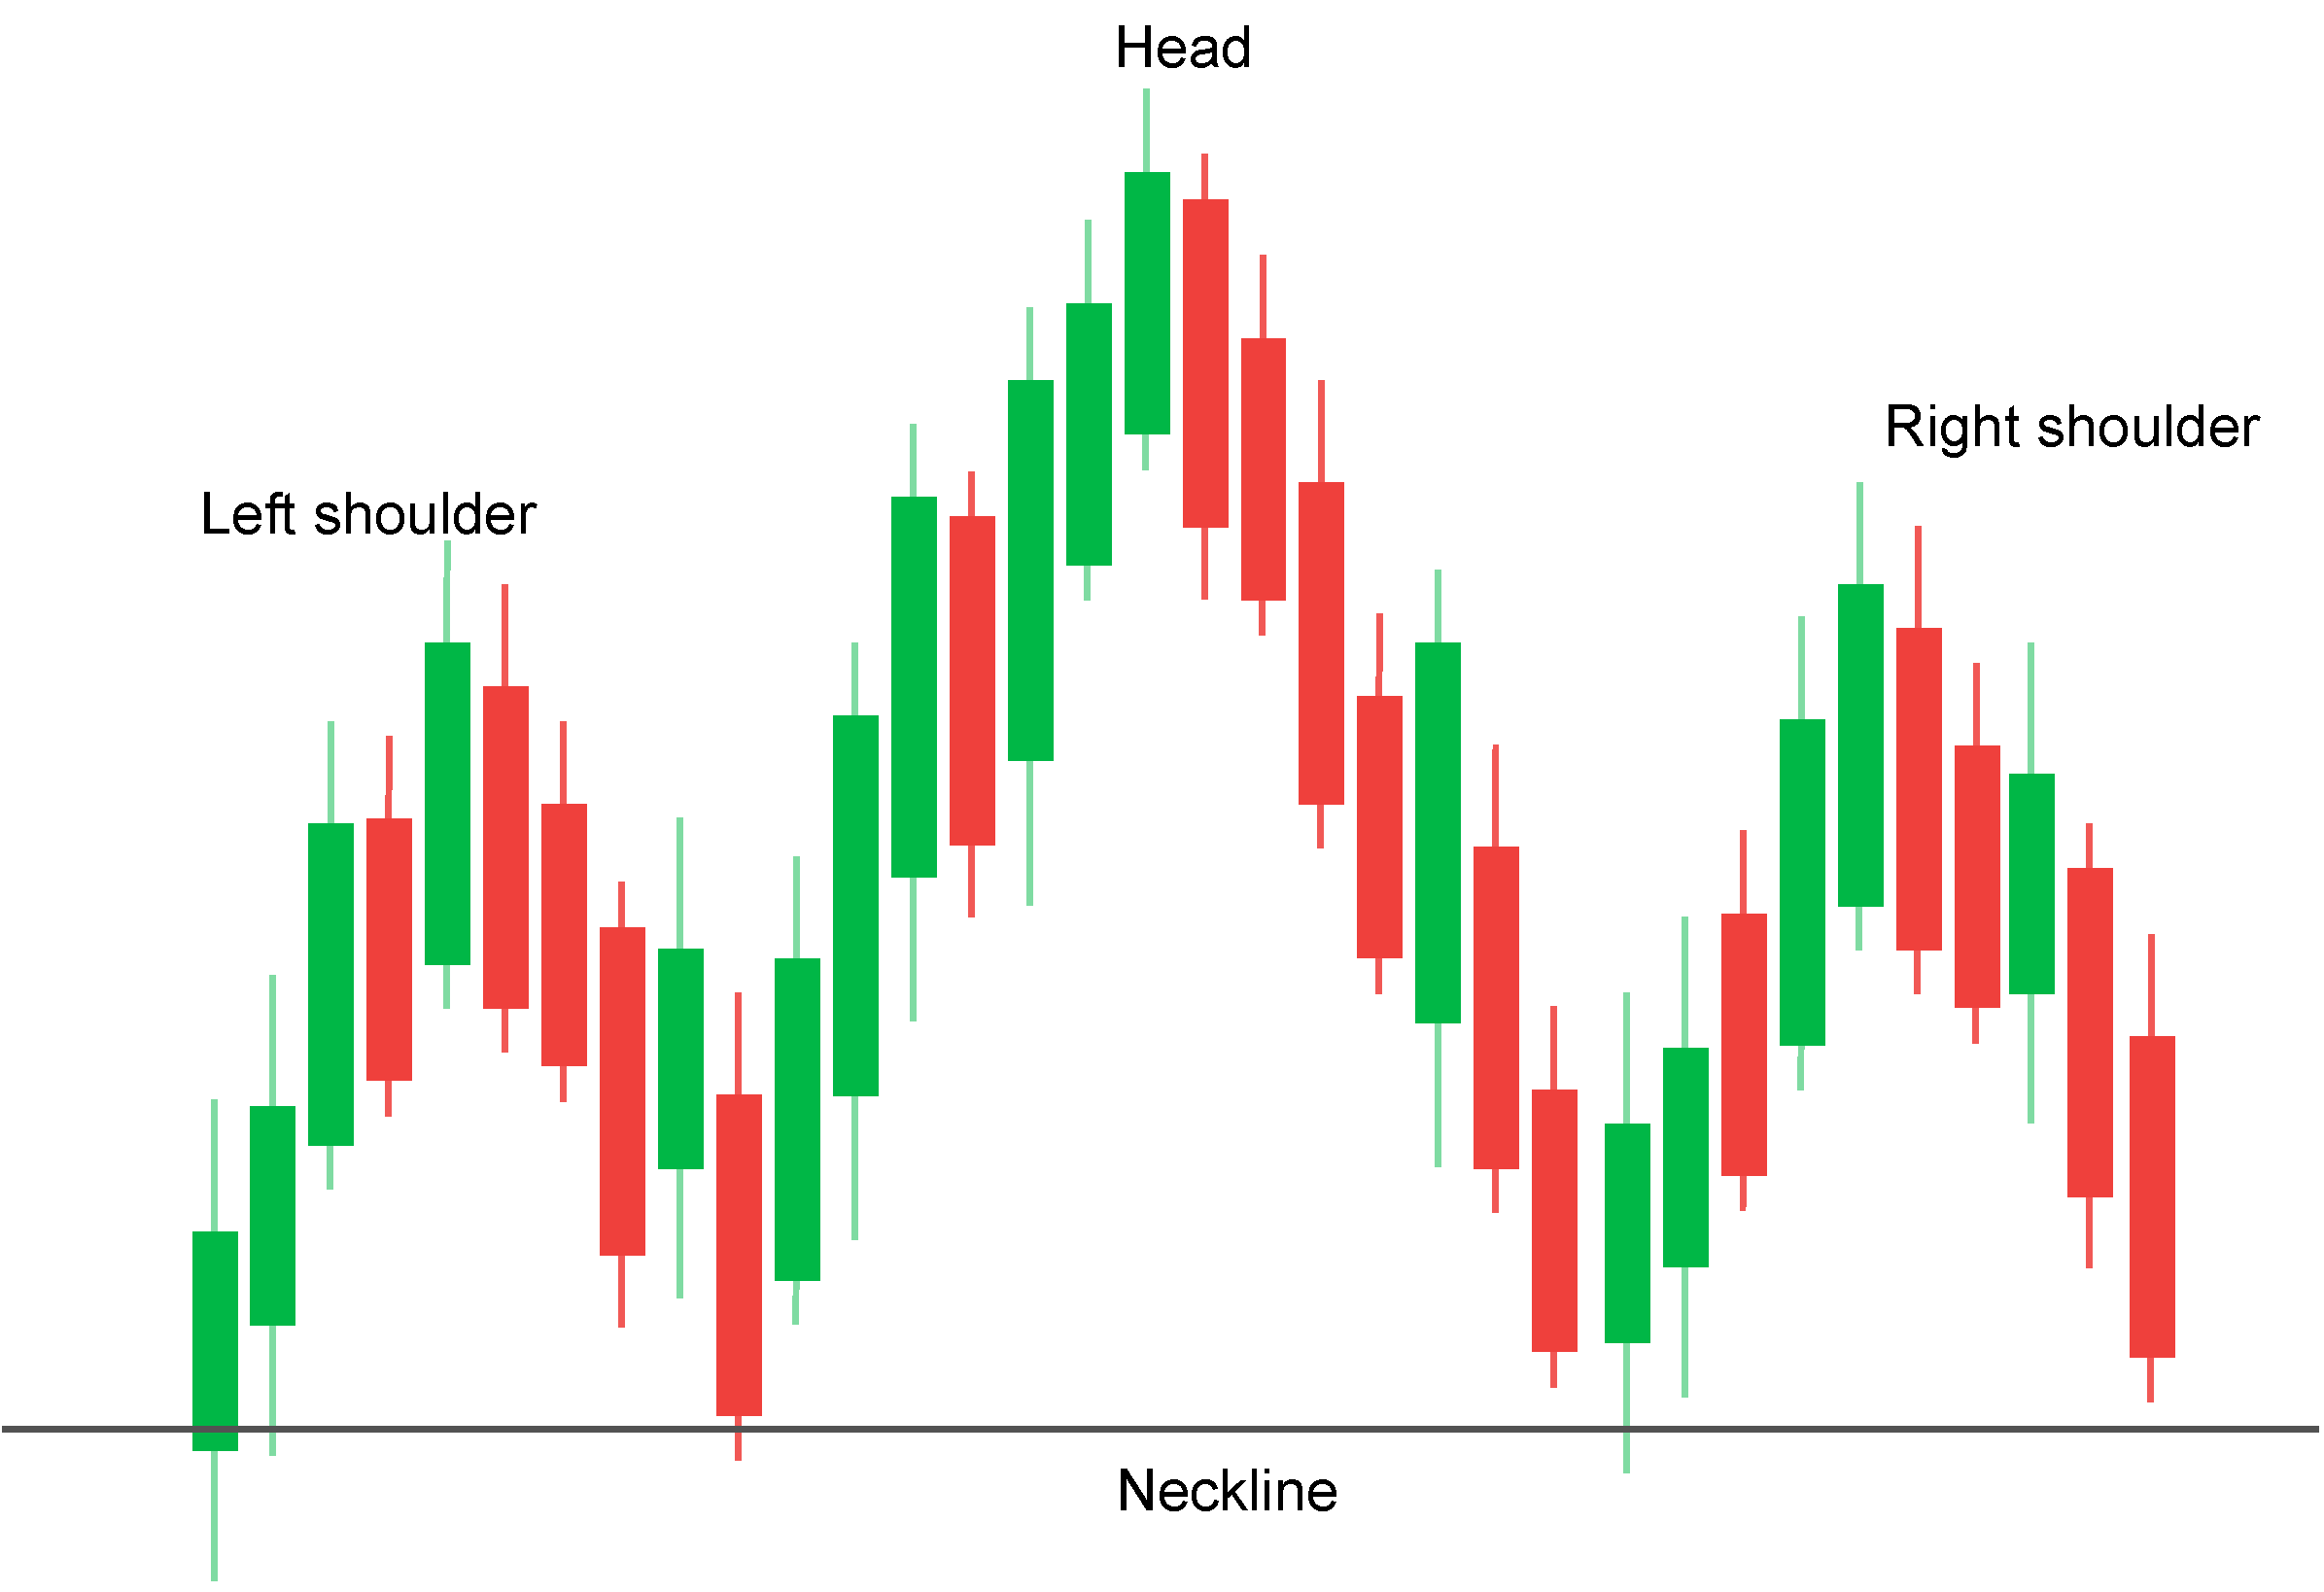
\includegraphics[width=0.7\textwidth]{Figures/Head-n-shoulders.pdf}
    \caption{Vzor \enquote{head and shoulders}}
    \label{fig:head-n-shoulders}
\end{figure}


\subsection{Cup and handle}
Formace připomínající šálek s rukojetí (obrázek \ref{fig:cup-n-handle}) je symbolem pro rostoucí trend na trhu. Identifikovatelný je tvorbou široké, ale ne příliš hluboké doliny, přičemž na končící ceně této doliny dojde k
dalšímu, již méně razantnímu poklesu v ceně. Tento menší pokles připomíná právě onu rukojeť a musí vždy následovat až po šálku. Toto pořadí je nezaměnitelné. Dolina by měla své dno
zaoblené a připomínat například misku. Šálek ve tvaru \enquote{V} není platným ukazatelem nastávajícího vzoru. Objem obchodů je relativně nízký, ale v období tvorby rukojeti se rapidně zvyšuje.
\begin{figure}[htb]
    \centering
    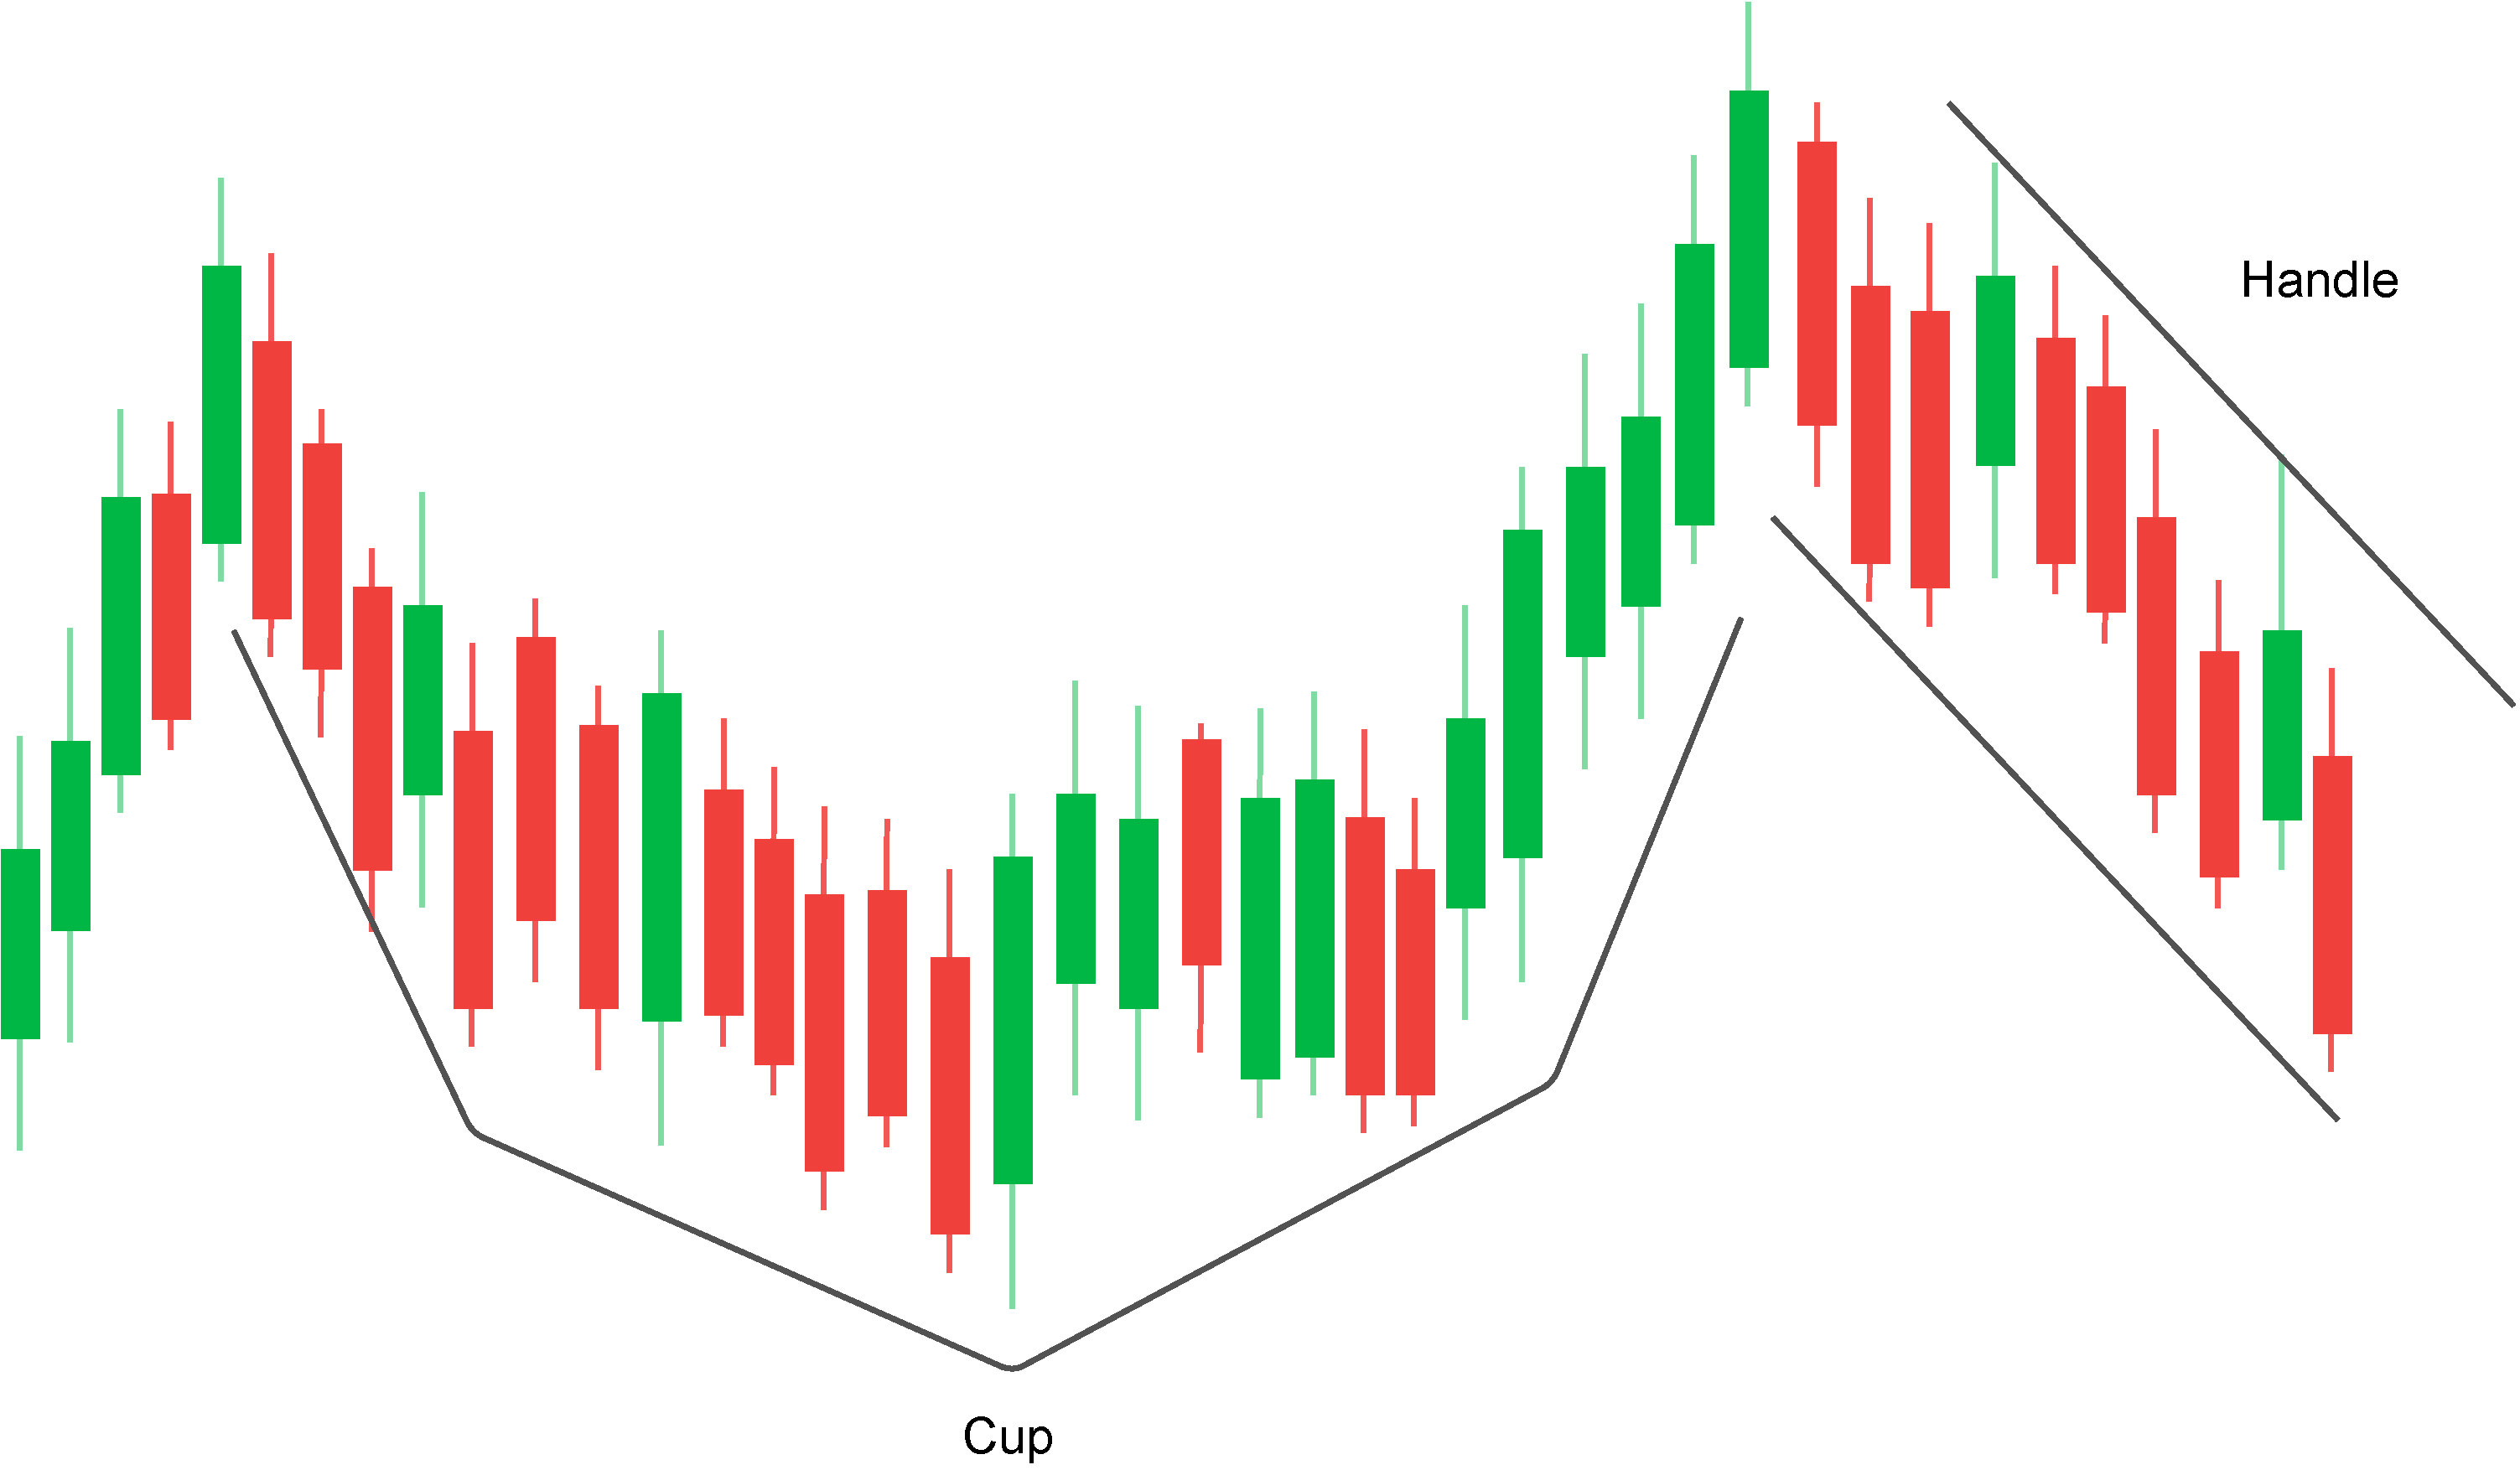
\includegraphics[width=0.7\textwidth]{Figures/Cup-n-handle.pdf}
    \caption{Vzor \enquote{cup and handle}}
    \label{fig:cup-n-handle}
\end{figure}

\subsection{Double top a Double bottom}
Další obratový vzor je \enquote{Double top}, vyskytující se na konci býčího trhu.\footnote{Označení popisující dlouhodobě stoupající cenový trend. Jeho opakem je medvědí trh pro označení
    dlouhodobě klesajícího trendu.} Po jasném potvrzení vzoru lze předpokládat pokles hodnoty aktiva. Opačným vzorem je Double bottom, formující se právě na konci medvědího trhu
s odhadem následně rostoucího cenového trendu. Double top je na grafu rozpoznatelný podle 2 kopců, zhruba ve stejné cenové úrovni, oddělené dolinou. Ona minimální cena v dolině
tvoří neckline tohoto vzoru. Jakmile je neckline proražena při sestupu z druhého kopce, je formace dokončena potvrzující signál k prodeji nebo shortování (viz \ref{subsubsec:positions}). Časové rozmezí mezi
kopci je taktéž rozhodující faktor při indikaci změny trendu. Jestliže se zformované kopce nacházejí v přibližně stejné cenové hladině, ale jsou časově příliš blízko sebe, může se jednat
pouze o konsolidaci trendu a jeho následné pokračování.
V případě Double bottom je formace překlopená, tedy se v ní vyskytují 2 doliny oddělené kopcem tvořící neckline. Oba útvary jsou znázorněná na obrázku \ref{fig:double-top}
\begin{figure}[htb]
    \centering
    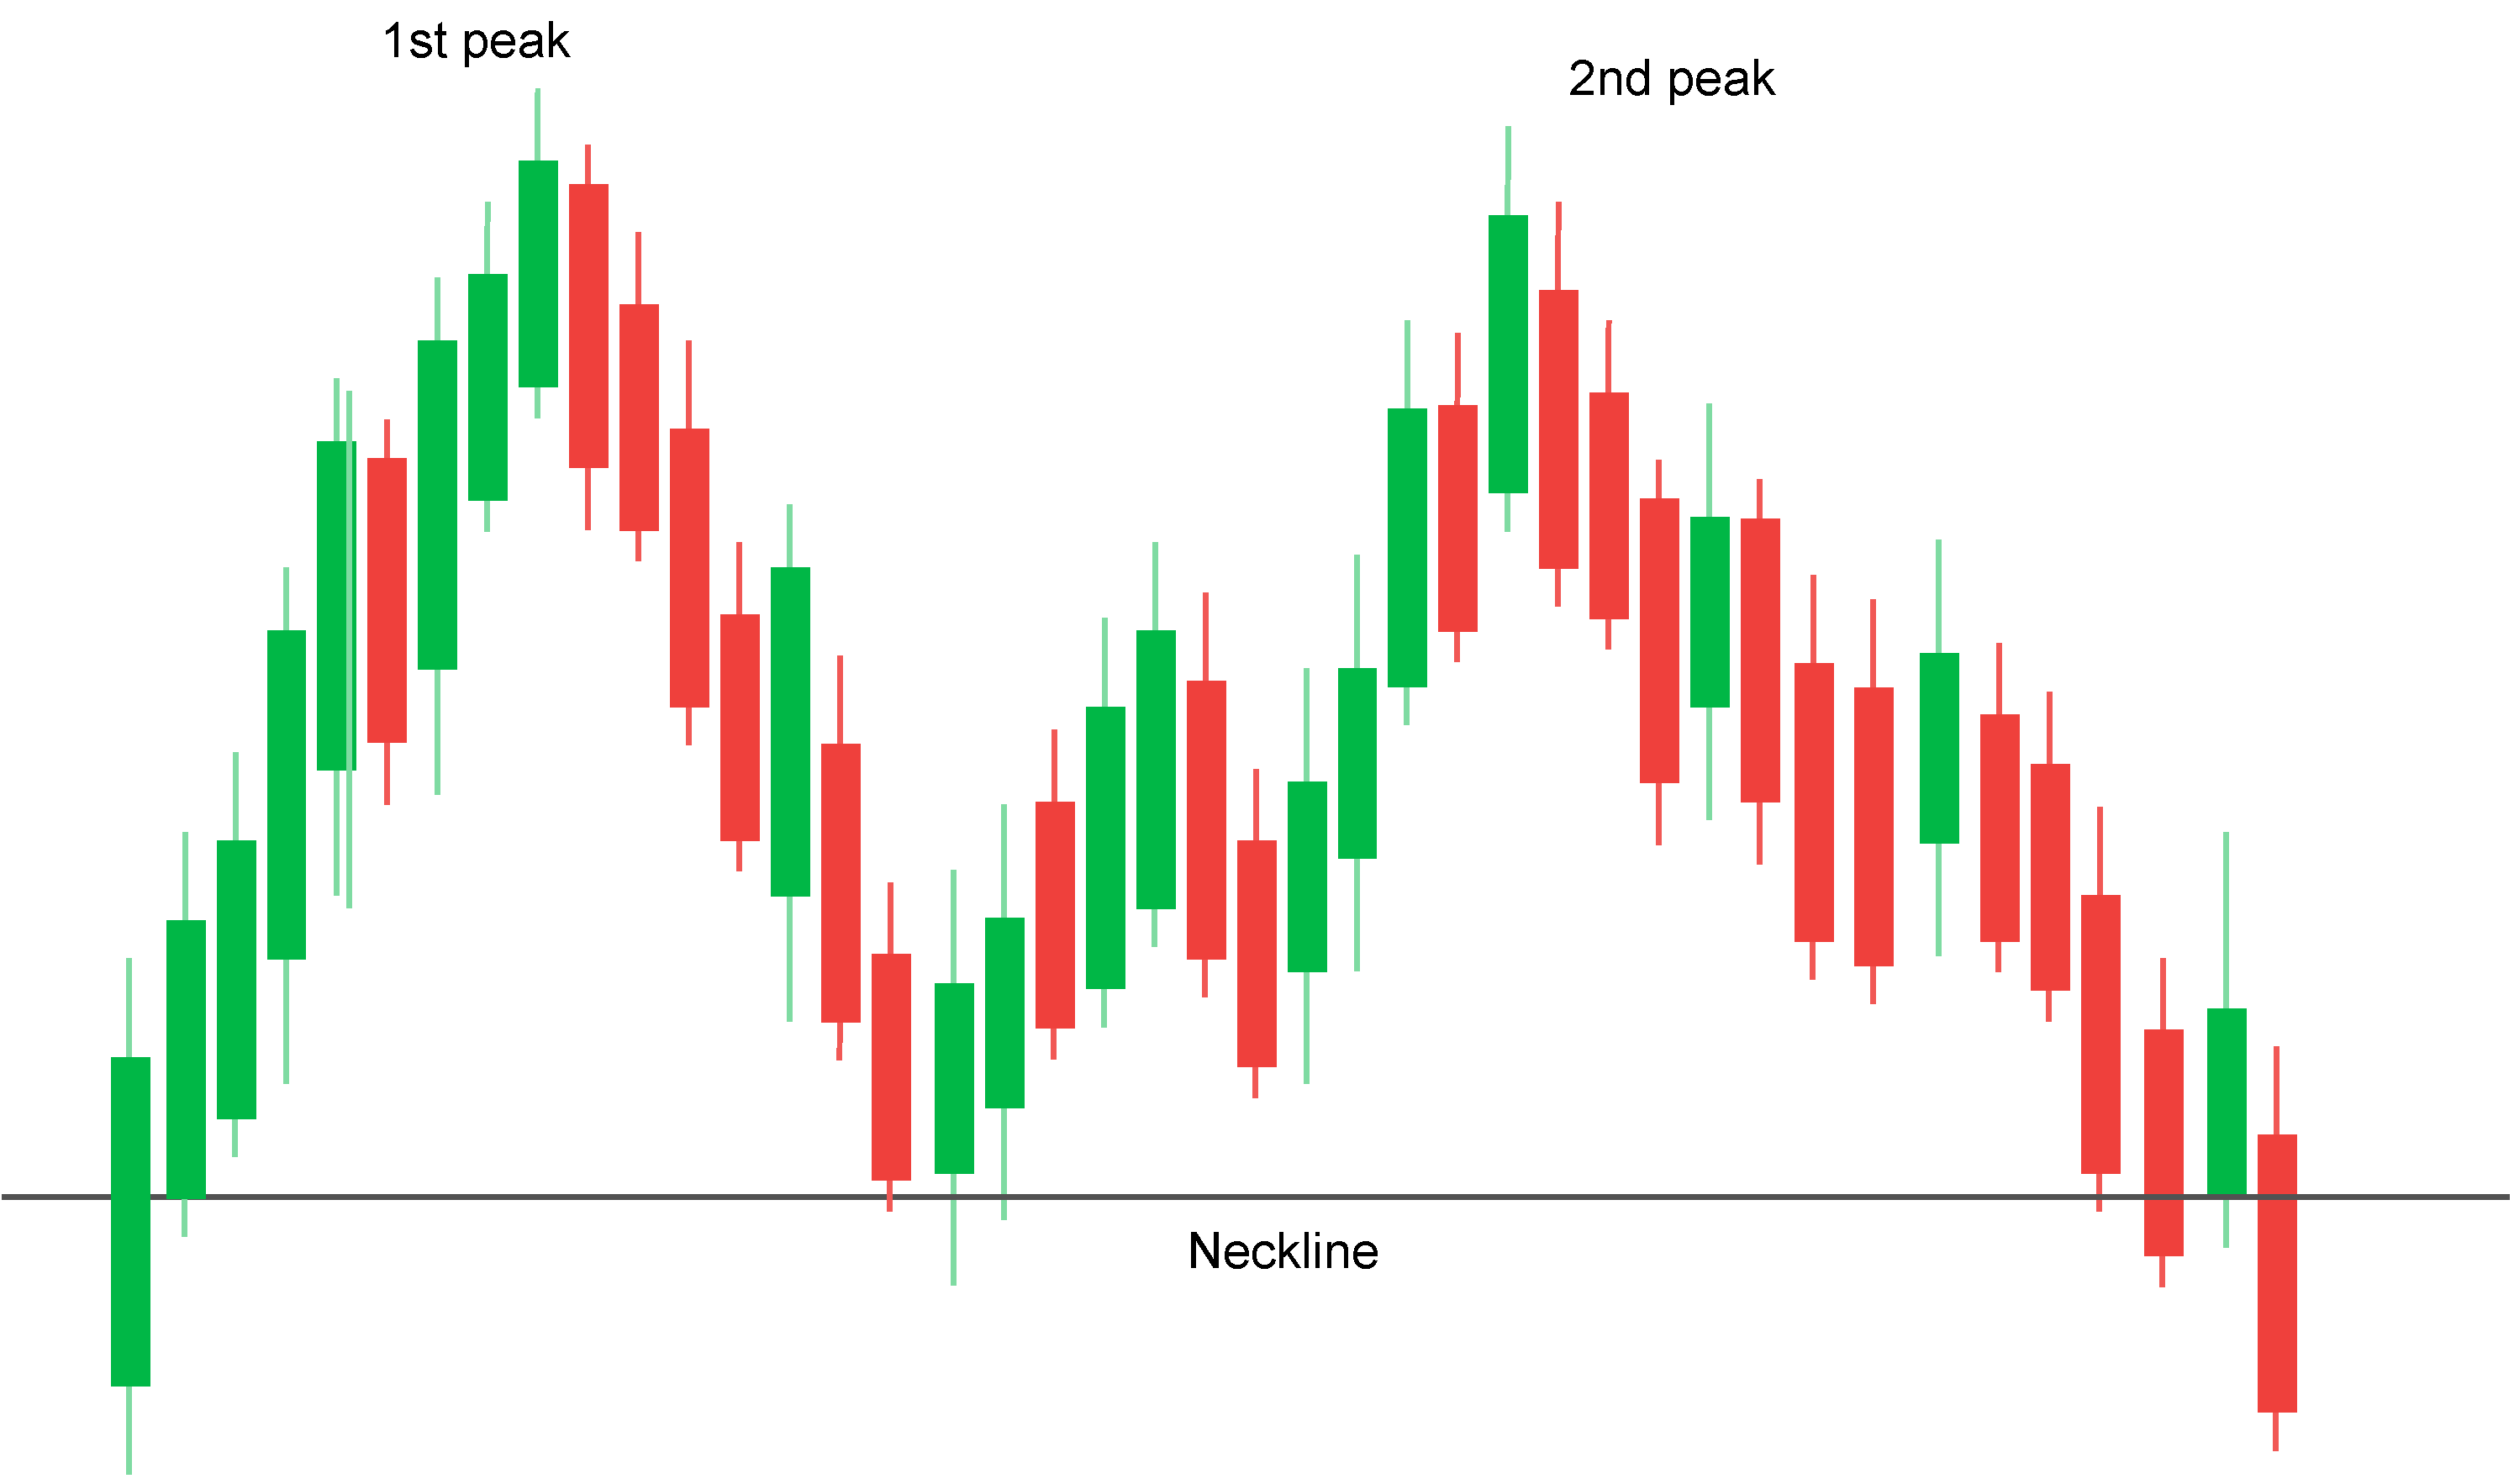
\includegraphics[width=0.6\textwidth]{Figures/double-top.pdf}
    \caption{Vzor \enquote{double top}}
    \label{fig:double-top}
\end{figure}

\subsection{Triple top}
Méně častý vzor Triple top, tvořený 3 kopci, slouží jako indikátor možné změny aktuálního tržního trendu. Pravidla potvrzení Triple topu jsou podobná jako u předchozího vzoru, tedy
kopce jsou na stejné cenové hladině, oddělující doliny (tvořící neckline). Jakmile dojde k proražení neckline, je formace dokončena. \ref{fig:triple-top}
\begin{figure}[htb]
    \centering
    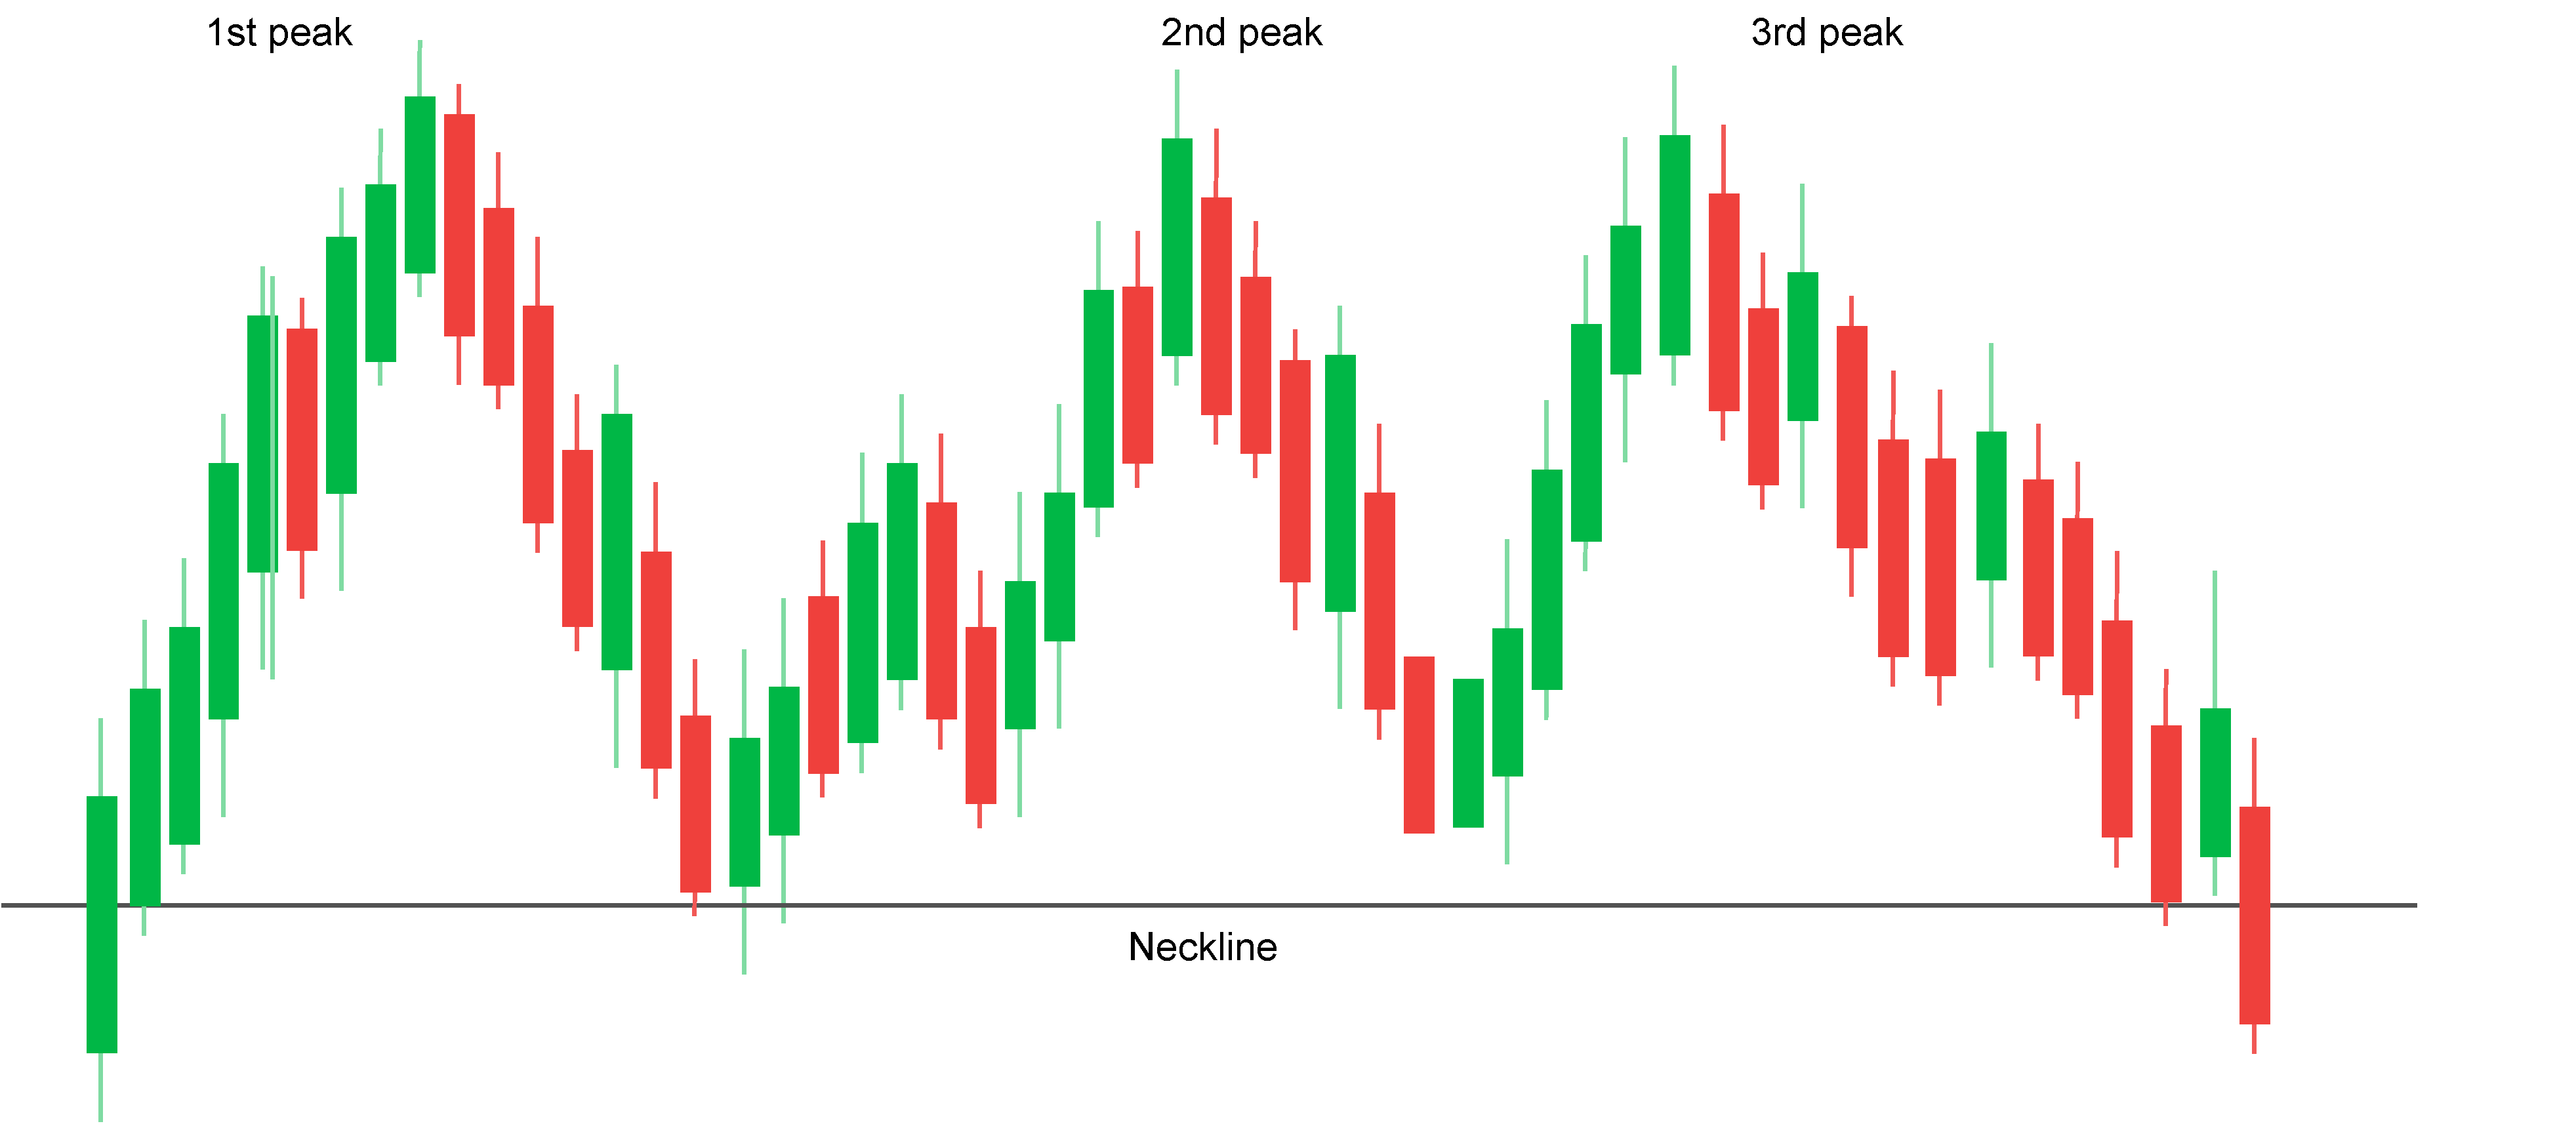
\includegraphics[width=0.7\textwidth]{Figures/triple-top.pdf}
    \caption{Vzor \enquote{triple top}}
    \label{fig:triple-top}
\end{figure}

\subsection{Wedge}
Wedge (klín) existuje ve dvou variantách, Falling wedge (padající klín) a Rising wedge (stoupající klín). Rozeznatelný je tím, že se svíčky pohybují v rozmezí dvou sbíhajících přímek.
Pokud je průsečík přímek pod momentální tržní cenovou hladinou, bude se jednat o padající klín. Naopak, jestliže je průsečík nad aktuální hodnotou aktiva, zformuje se stoupající klín.
Význam, který tento vzor poskytuje se liší na základě trendu a utvořené varianty.
\begin{figure}[ht]
    \centering
    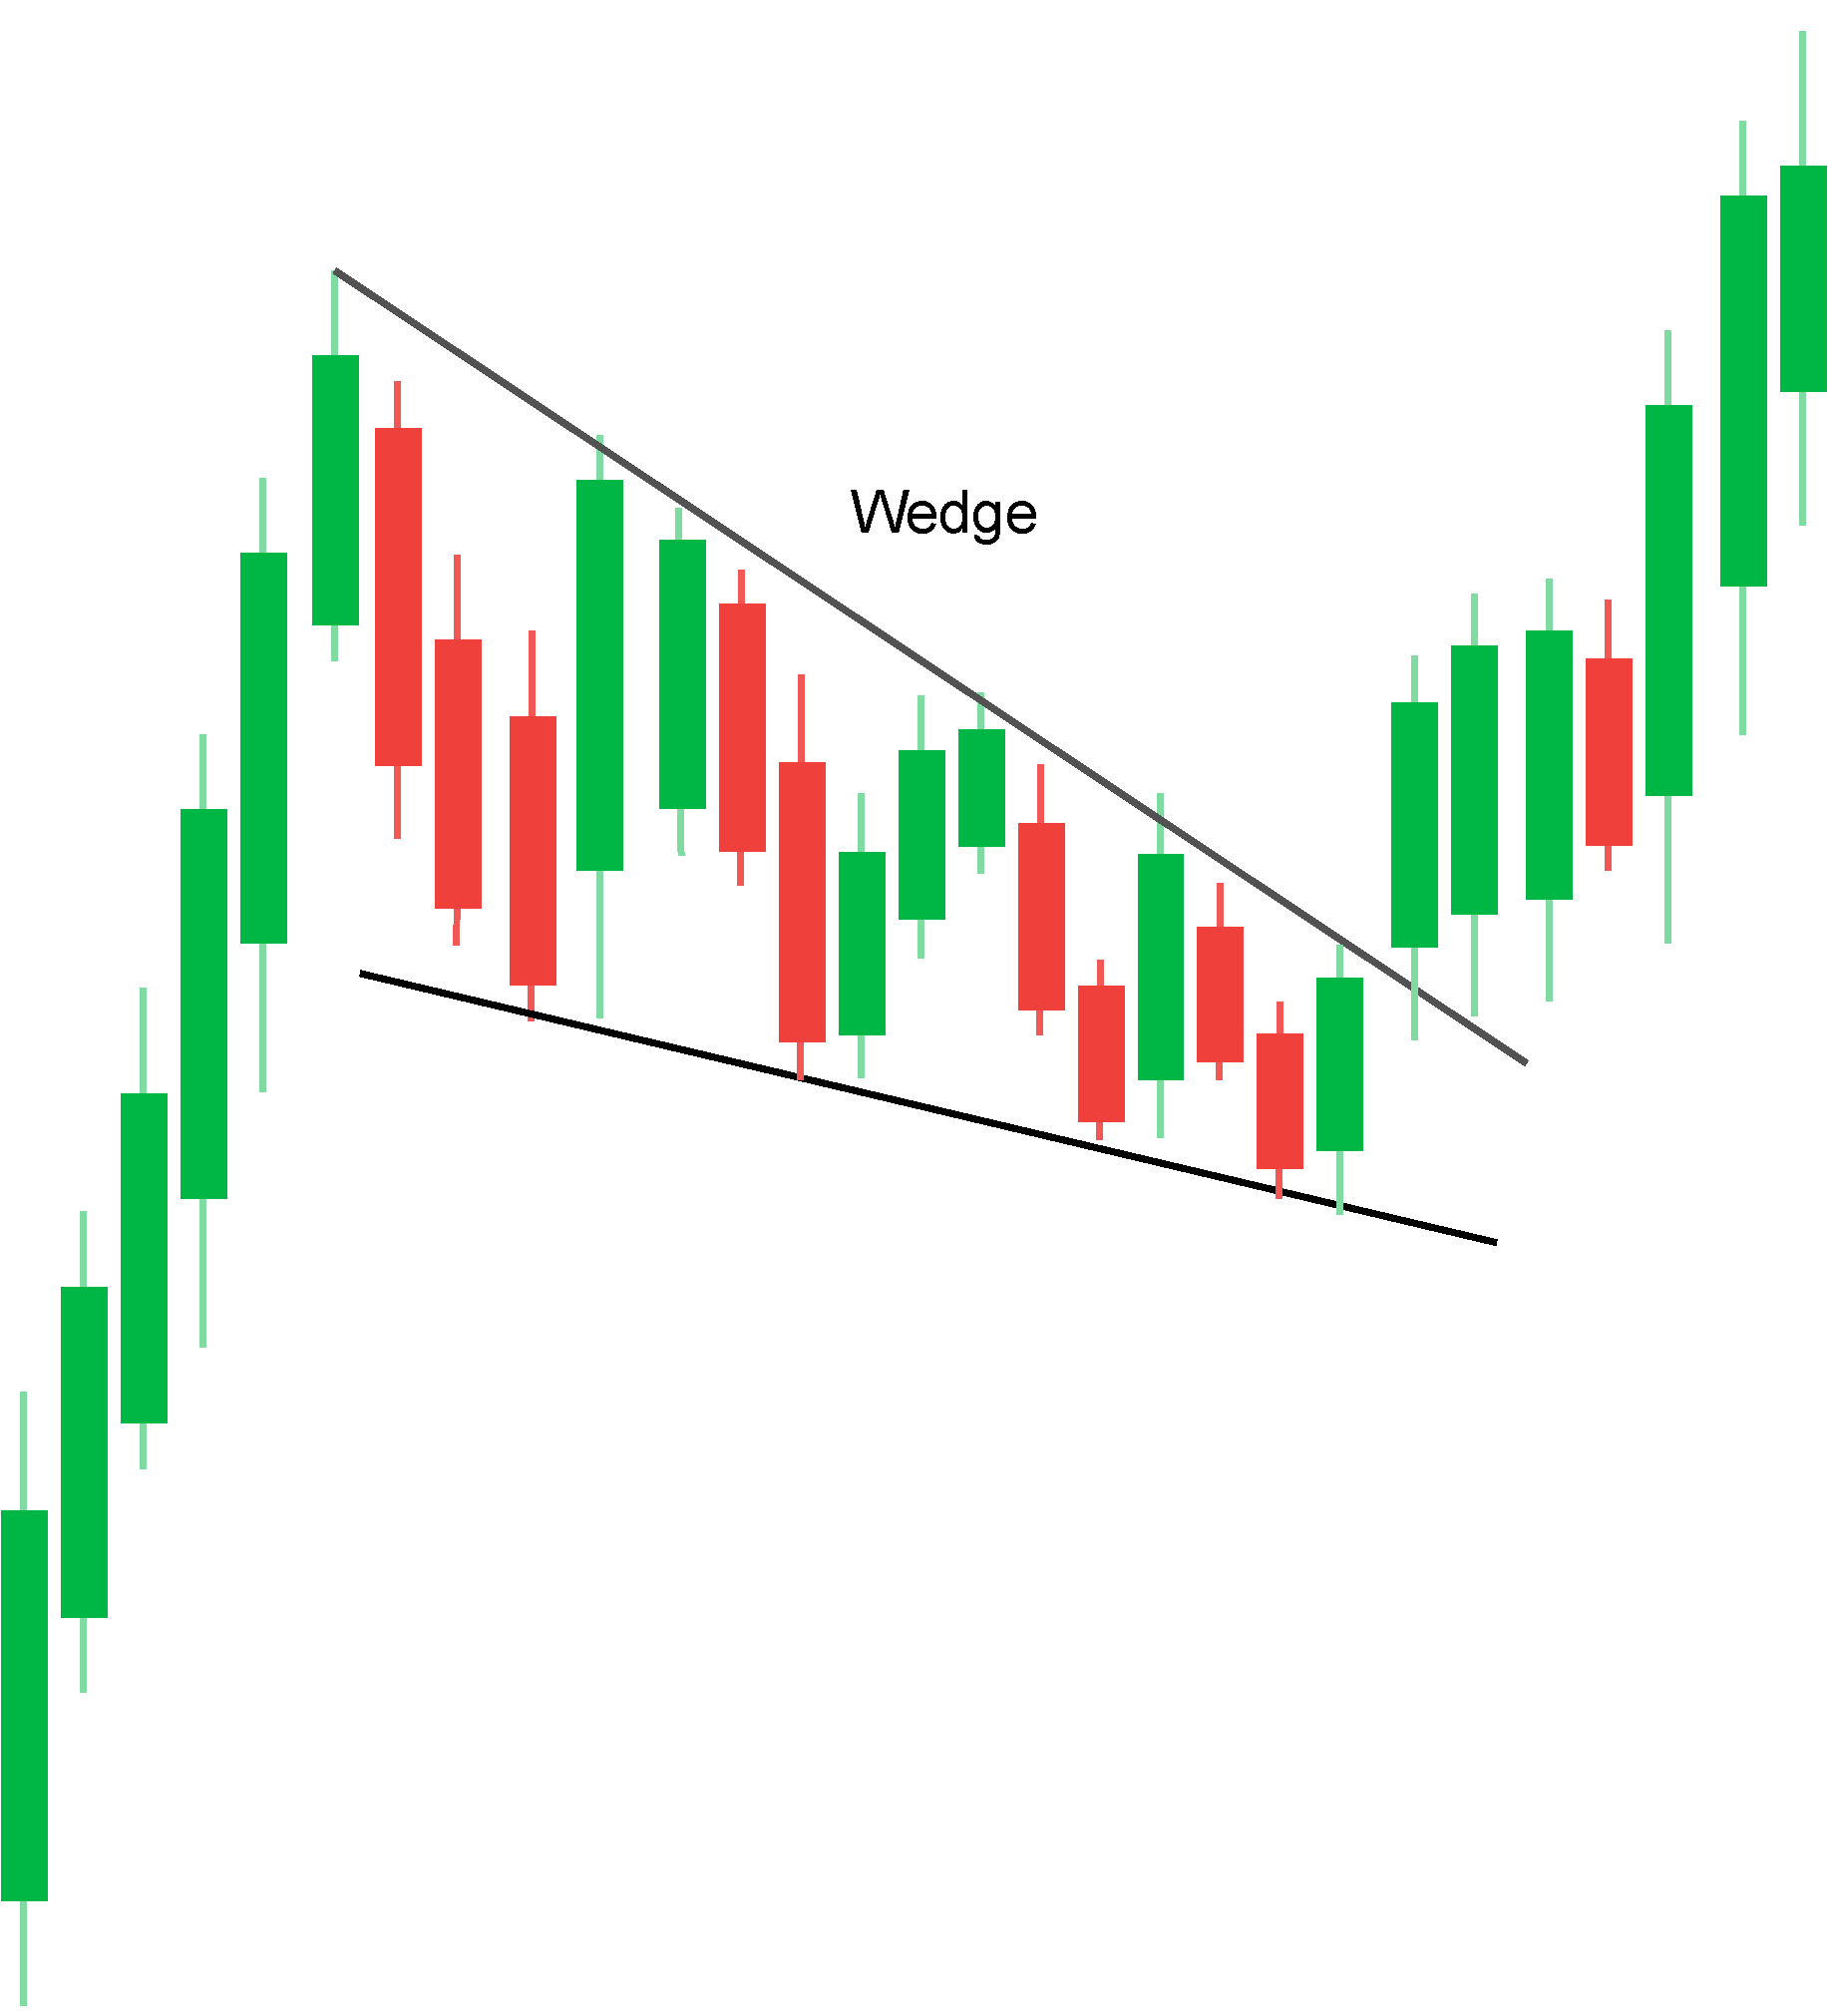
\includegraphics[width=0.6\textwidth]{Figures/wedge.pdf}
    \caption{Vzor \enquote{wedge}}
    \label{fig:wedge}
\end{figure}

\emph{Padající klín} v sestupném trendu signalizuje obrat, jelikož smršťování cenových rozsahů značí, že trend ztrácí sílu. Nalezení tohoto vzoru ve vzestupném trendu indikuje pouze
dočasné pozastavení. Trh se trochu zkoriguje, a původní trend bude pokračovat. Velikost obchodů v tomto vzoru se společně s množstvím obchodů snižuje kvůli zmenšujícím se cenovým
rozsahům. Jakmile dojde k průrazu, začnou se parametry obchodů opět odrážet aktuální trend. \ref{fig:wedge}

\emph{Stoupající klín} indikuje podobné signály jako padající klín. Pokud je nalezen při vzestupném trendu, je velice pravděpodobné, že bude následovat obrat trendu. V případě, že jej
nalezneme v klesajícím trhu, bude to náznak spíše korekce a klesání bude pokračovat.

\subsection{Triangle}
Posledním uvedeným vzorem je trojúhelník (\ref{fig:triangle}). Oproti klínu se liší v tom, že jedna z přímek je vždy zarovnaná a tvoří cenovou hladinu, od které se svíčky odráží zpět. Tento vzor, stejně
jako klín, má stoupající a klesající variantu. Stoupající trojúhelník se formuje ve chvíli, kdy trh v daném časovém okně zaznamenává vyšší minima, ale maxima se zachovávají stejně vysoká.
Pro klesající trojúhelník je situace opačná - maxima se krok za krokem snižují a minima zůstávají na stejné úrovni. Jestliže narazíme na stoupající trojúhelník při vzestupném trendu,
můžeme očekávat pokračování tohoto trendu. Avšak nalezneme-li jej v trendu sestupném, může se jednat o silnou indikaci obratu tržní nálady.
\begin{figure}[ht]
    \centering
    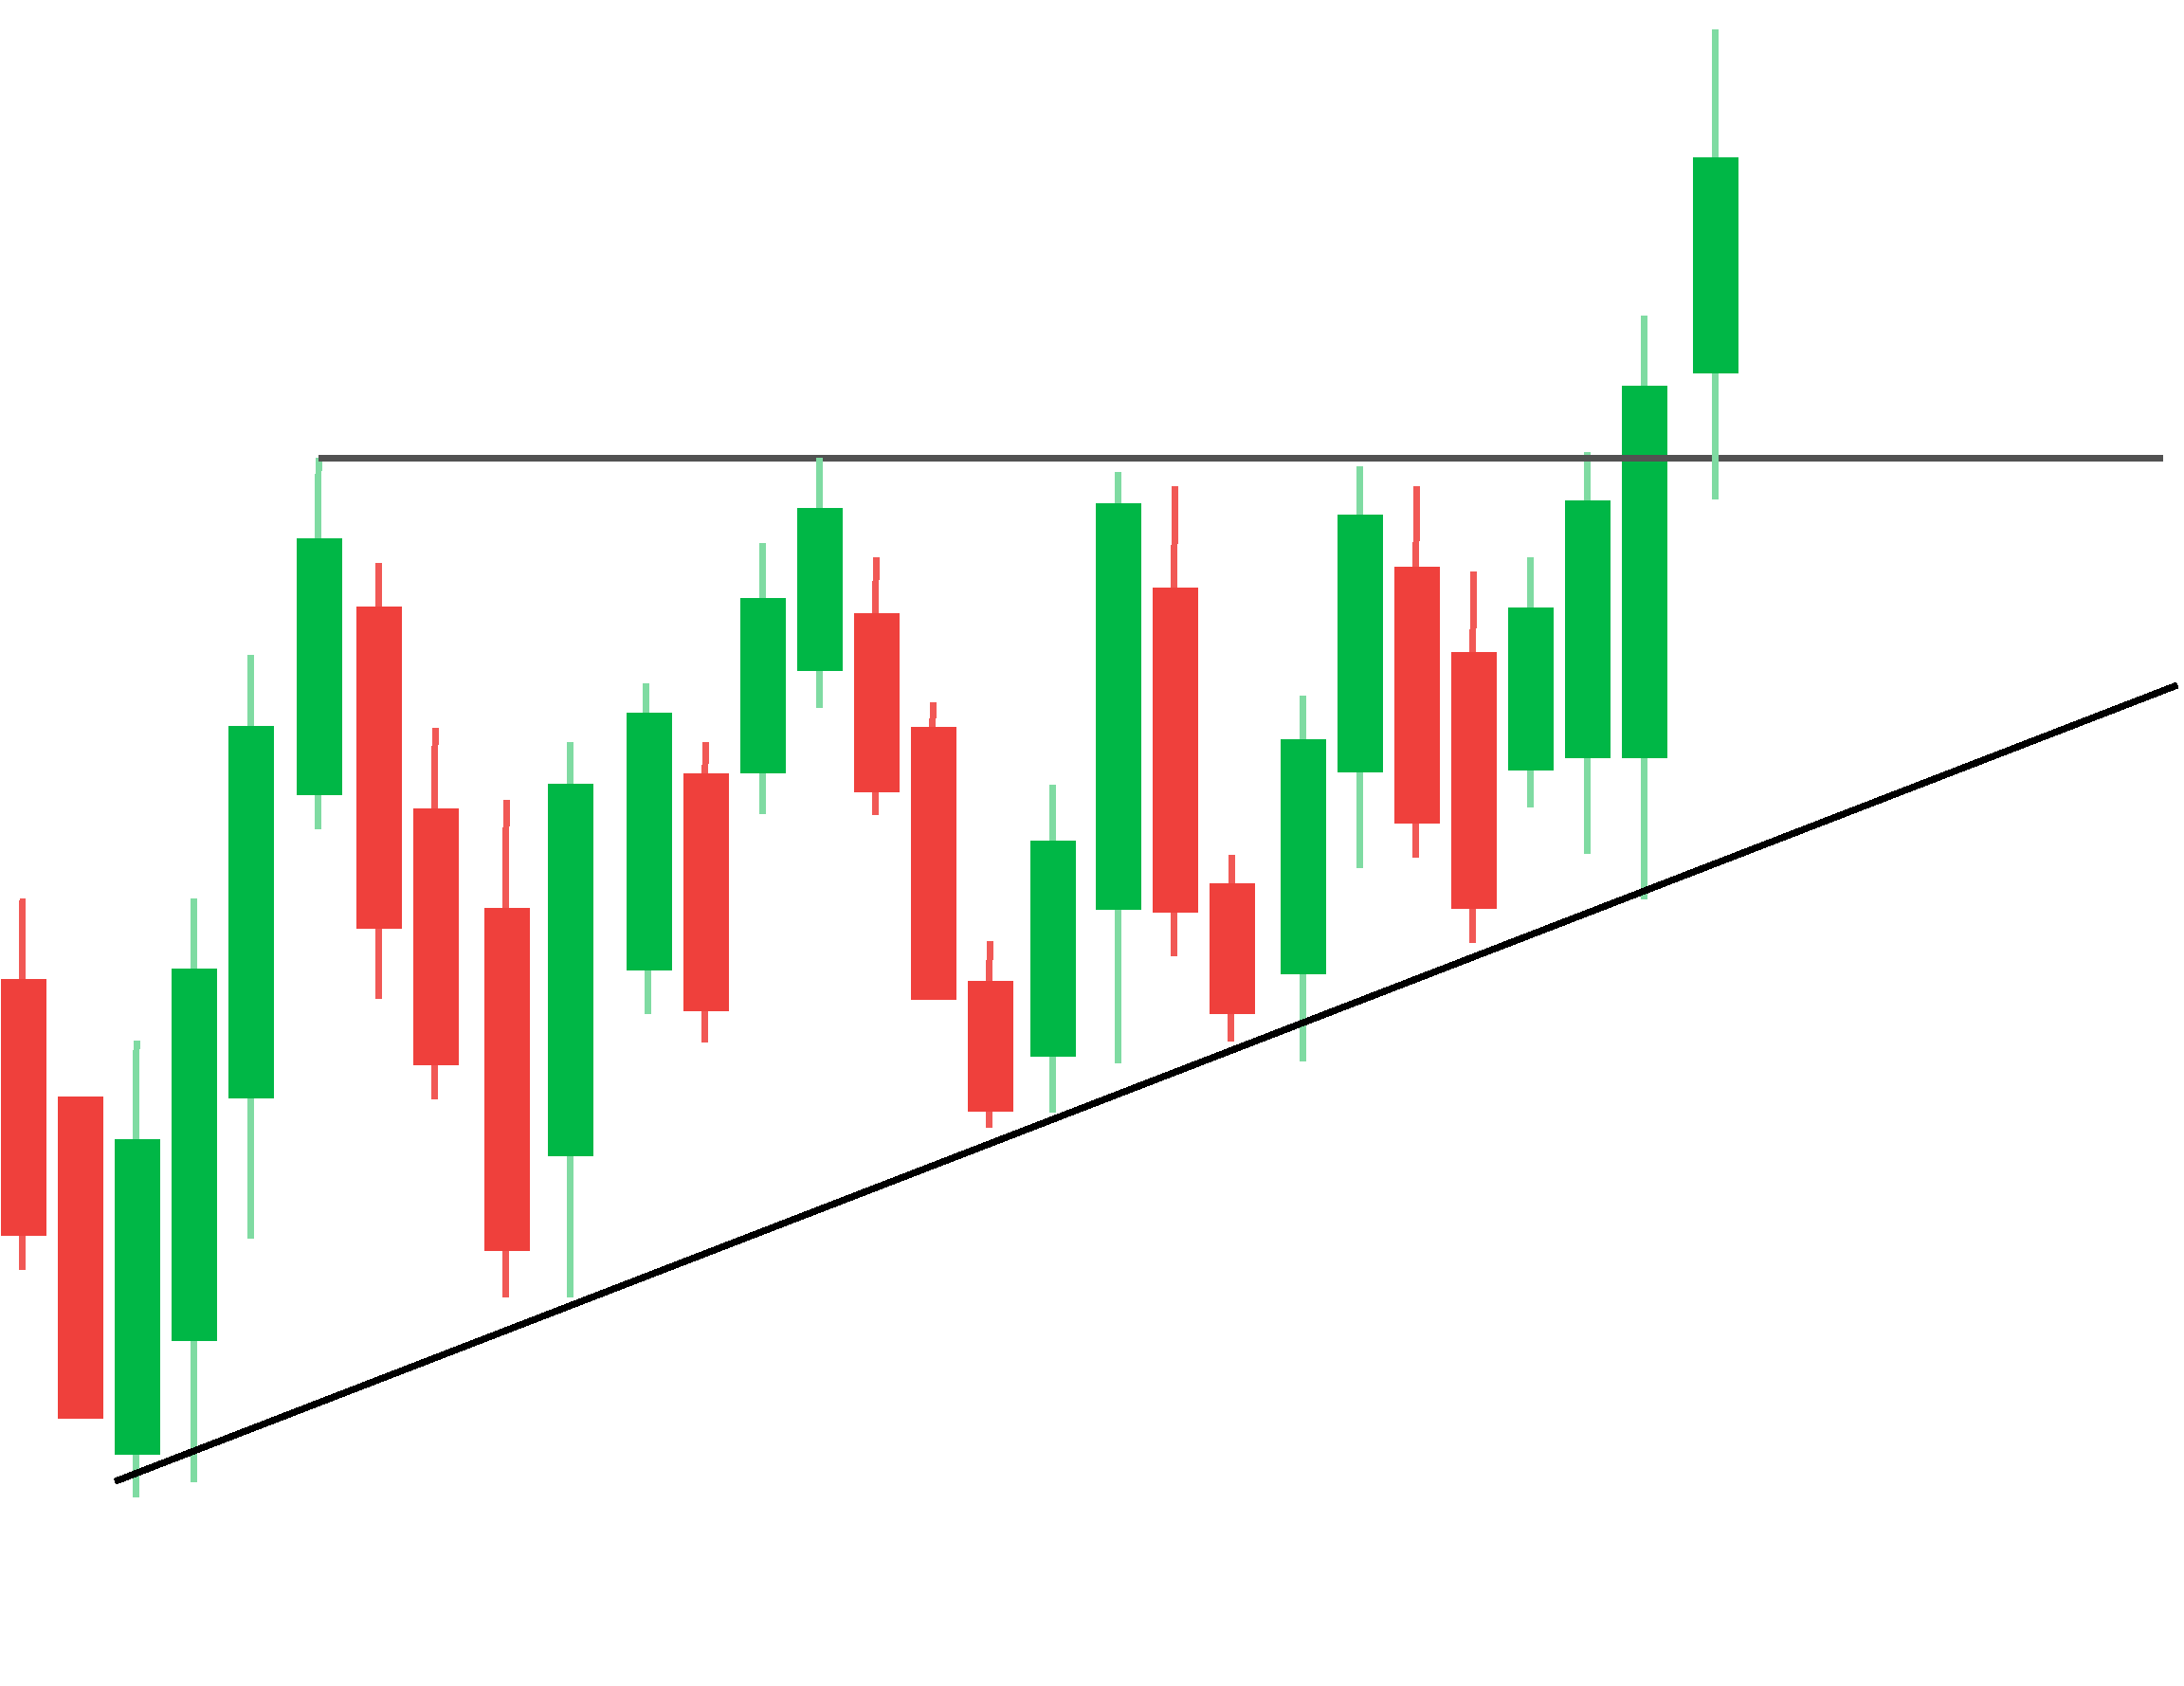
\includegraphics[width=0.6\textwidth]{Figures/triangle.pdf}
    \caption{Vzor \enquote{triangle}}
    \label{fig:triangle}
\end{figure}

\clearpage
\newpage


\section{Support a resistance}
\label{sec:TrendingLines}
V předchozí sekci zabývající se grafovými vzory se několikrát objevily určité čáry, od kterých se tržní cena odrážela zpět nahoru nebo naopak dolů. Tyto čáry se též označují jako odporové
úrovně \emph{support} a \emph{resistance}. Support je cenová úroveň, od které se ceny \enquote{odrážejí} když klesají dolů. To znamená, pokud existuje posloupnost svíček, jejichž close cena
klesá, jakmile se přiblíží k ceně supportu tak se spíše odrazí a cena aktiva začne opět stoupat. Naopak k tomu resistance je hranice, která tvoří \enquote{zábranu} stoupajícím cenám.
V momentě kdy se svíčky blíží úrovně rezistence je velká pravděpodobnost že se odrazí a dojde ke klesání.

Existuje několik způsobů jak identifikovat tyto odporové úrovně. Nejčastější metoda je s pomocí trendových čar. Trendové linie se jednoduše zakreslí spojením spodních a horních stínů svíček.
Čím více jsou tyto úrovně otestovány tím, že se cena od nich odráží, tím větší význam můžeme těmto úrovním skutečně připsat. Jakmile dojde k proražení rezistance, stává se ona úroveň
supportem. Pravdivý je i opačný případ, kdy dojde k proražení supportu a stává se z toho nová rezistance.
Pokud se cena aktiva pravidelně pohybuje v těchto úrovních, nejjednodušší využití tohoto cyklu je nakupovat, když se cena pohybuje v blízkosti supportu a prodávat v okolí rezistance.
Samozřejmě je důležité uvážit časové okno pro zakreslování těchto úrovní a doba obchodování.

\section{Indikátory}
\label{sec:Indicators}
Indikátory jsou signifikantní součástí technické analýzy \cite{stock:analysis}. Technické indikátory se opírají o matematické výpočty a počítají se za nějaké období. Jako vstupem do výpočtu se nejčastěji
bere tržní cena nebo objem obchodů. Na základě těchto informací jsou dané výstupy, které dodávají další informace k obchodování.
Obecně se technické indikátory dělí na indikátory hybnosti (momentum indikátory), trendové indikátory a oscilátory. Momentum indikátory měří dynamiku ceny, tedy rychlost změny.
Trendové indikátory se zaměřují na odhad aktuálního trendu a případnou predikci jeho otočení. Jako oscilátory se označují indikátory, které se pohybují v daném rozmezí (např. -1 až 1).
Tato sekce se zabývá několika nejpoužívanějšími technickými indikátory, rozebírá způsob jejich výpočtu a dodanou informační hodnotu. Pro následující rovnice znázorňující výpočet indikátoru
vždy platí, že $C$ se značí \emph{close} cena období.

\subsection{Indikátor objemu (OBV, On-balance volume)}
Jedná se o kumulativní indikátor objemu obchodů. Měří nákupní a prodejní tlak a spojuje tržní cenu v závislosti na velikostech obchodů. Pokud se OBV zvyšuje, více obchodníků
je ochotných zaplatit za aktivum v jeho momentální tržní ceně. Pokud je trh ve vzestupném trhu a navíc k tomu stoupá i hodnota tohoto indikátoru, potvrzuje se tímto onen trend.
Jestliže cena stoupá, ale hodnota OBV nijak neroste, je trh spíše zmatený. Výpočet OBV je znázorněn ve vzorci \ref{eq:obv} a vizualizace na obrázku \ref{fig:obv}.

\begin{equation}
    OBV_t = OBV_{t-1} +
    \begin{cases}
        objem, & C_t \ge C_{t-1} \\
        0,     & C_t = C_{t-1}   \\
        objem, & C_t \le C_{t-1}
    \end{cases}
    \label{eq:obv}
\end{equation}

\begin{figure}[h]
    \centering
    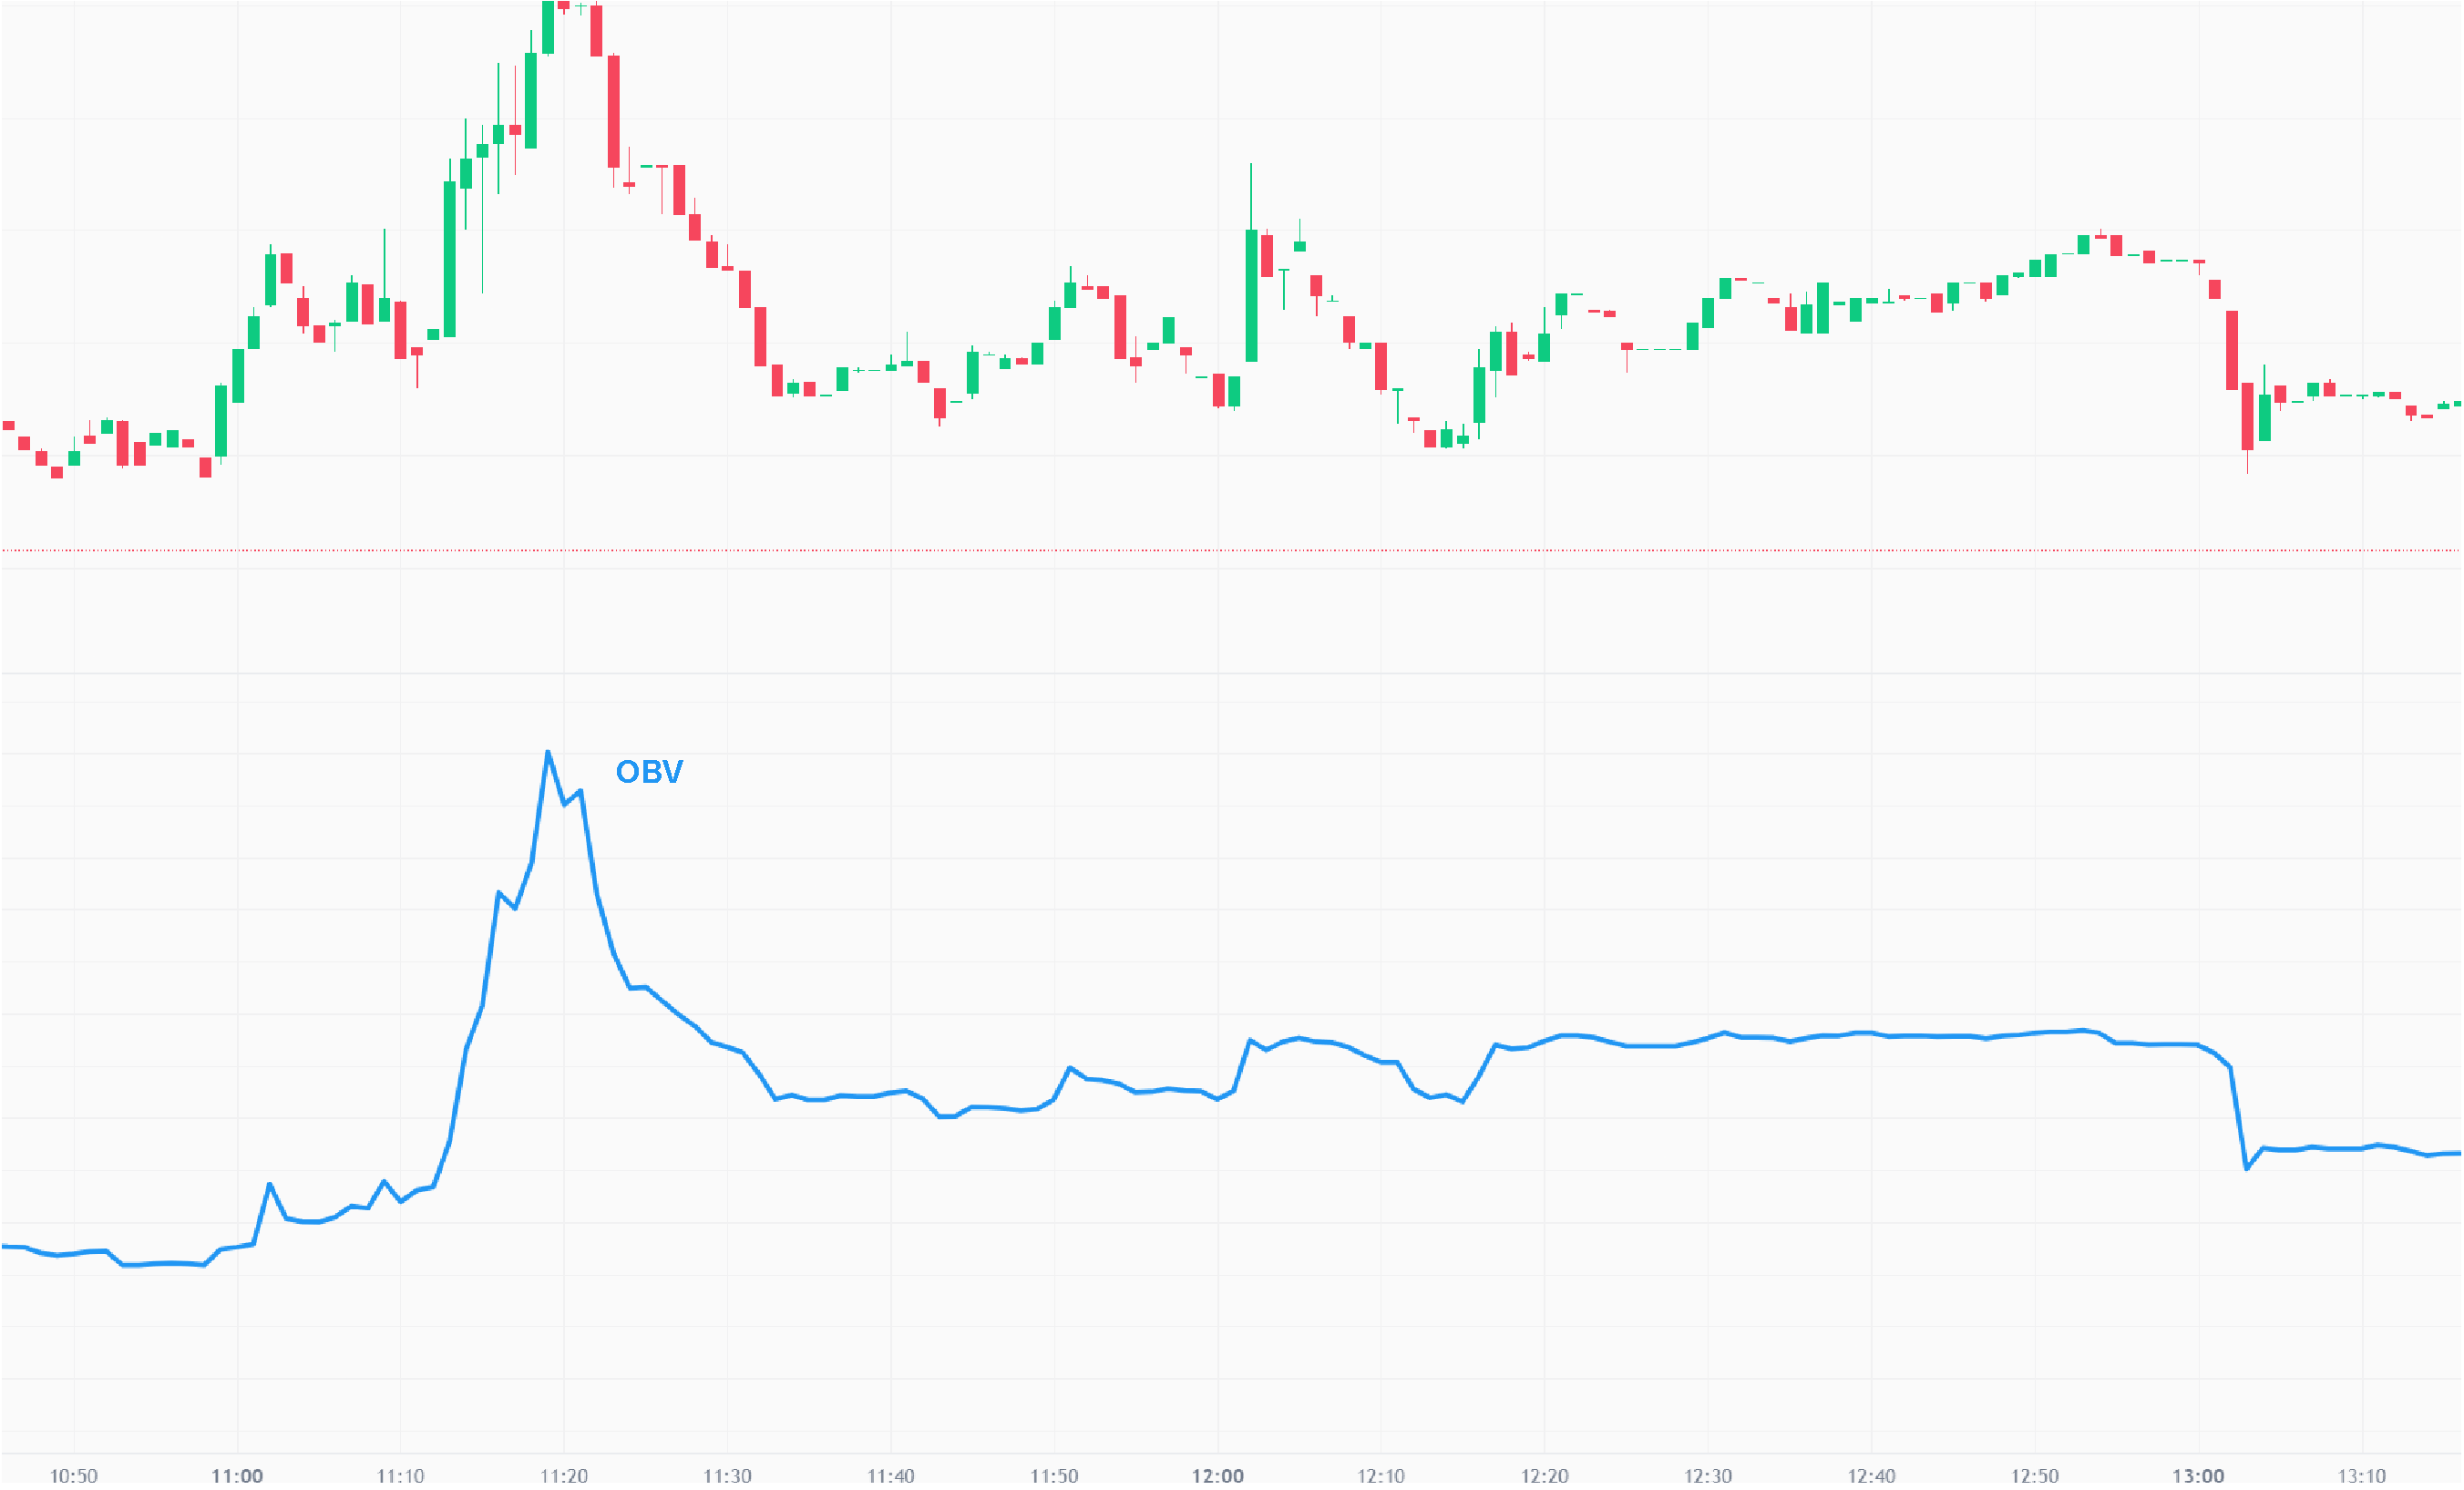
\includegraphics[width=1\textwidth]{Figures/OBV.pdf}
    \caption{Znázornění indikátoru OBV \cite{tradingview}}
    \label{fig:obv}
\end{figure}

\subsection{Klouzavý průměr (MA, Moving average)}
Klouzavý průměr má hned několik variant výpočtu. Klouzavý průměr se počítá pouze za určené období. Oblíbené časové úseky jsou 10, 40, nebo 200 dní zpětně.
Navzdory představě tento indikátor není \enquote{pouze jedno číslo}, ale celá série, jelikož průměr je počítán pro každý datový bod, tedy pro každou svíčku zvlášť. Propojením vypočítaných
hodnot vzniká na grafu linie představující plovoucí odporovou úroveň s výhodou jakési odolnosti proti krátkodobým fluktuacím v cenách aktiva. Tato odolnost usnadňuje predikci spíše dlouhodobějších trendů.
Jestliže se trh nachází v sestupném trendu, MA se chová jako úroveň rezistence a její proražení dává signál k nákupu, předpovídající vzestupný trend.
Opačný případ je taktéž pravdivý, kdy ve vzestupném trhu MA zastává roli supportu.

Dva nejpoužívanější typy výpočtu MA jsou \emph{Simple Moving Average (SMA)} a \emph{Exponential Moving Average (EMA)} (viditelné na obrázku \ref{fig:ma-sma-ema}).
SMA je jednoduchý pro výpočet a jedná se o obyčejný průměr na období
o velikosti \emph{n} a způsob výpočtu je vyobrazena ve vzorci \ref{eq:sma}. EMA využívá váženého průměru, ve kterém se váha starších datový bodů exponenciálně snižuje, a tím se preferují spíše novější hodnoty hladiny kurzu.
Při výpočtu tohoto váženého průměru se používá i takzvaný vyhlazovací koeficient $\alpha$, přičemž nejčastější nastavení tohoto koeficientu je $ \alpha = \frac{2}{n+1}$.
Rekurzivní metoda výpočtu lze vidět na vzorci \ref{eq:ema}. Pro pohyblivé časové okno lze využít druhou možnost výpočtu EMA viditelnou ve vzorci \ref{eq:ema-rolling}.
Výhodou exponenciálního klouzavého průměru je větší důraz na novější data, čím může lépe reagovat na změny trhu.

\begin{equation}
    SMA_t = \frac{C_t + C_{t - 1} + \cdots + C_{t - (n - 1)}}{n}
    \label{eq:sma}
\end{equation}

\begin{equation}
    EMA_t = \alpha * C_t + (1 - \alpha) * EMA_{t - 1}
    \label{eq:ema}
\end{equation}

\begin{equation}
    EMA_t = \frac{C_t + (1 - \alpha) * C_{t-1} + (1 - \alpha)^2 * C_{t-2} + \cdots + (1 - \alpha)^t * C_0}{1 + (1 - \alpha) + (1 - \alpha)^2 + \cdots + (1 - \alpha)^t}
    \label{eq:ema-rolling}
\end{equation}
% TODO: Pridat ukázky SMA a EMA

\begin{figure}[h]
    \centering
    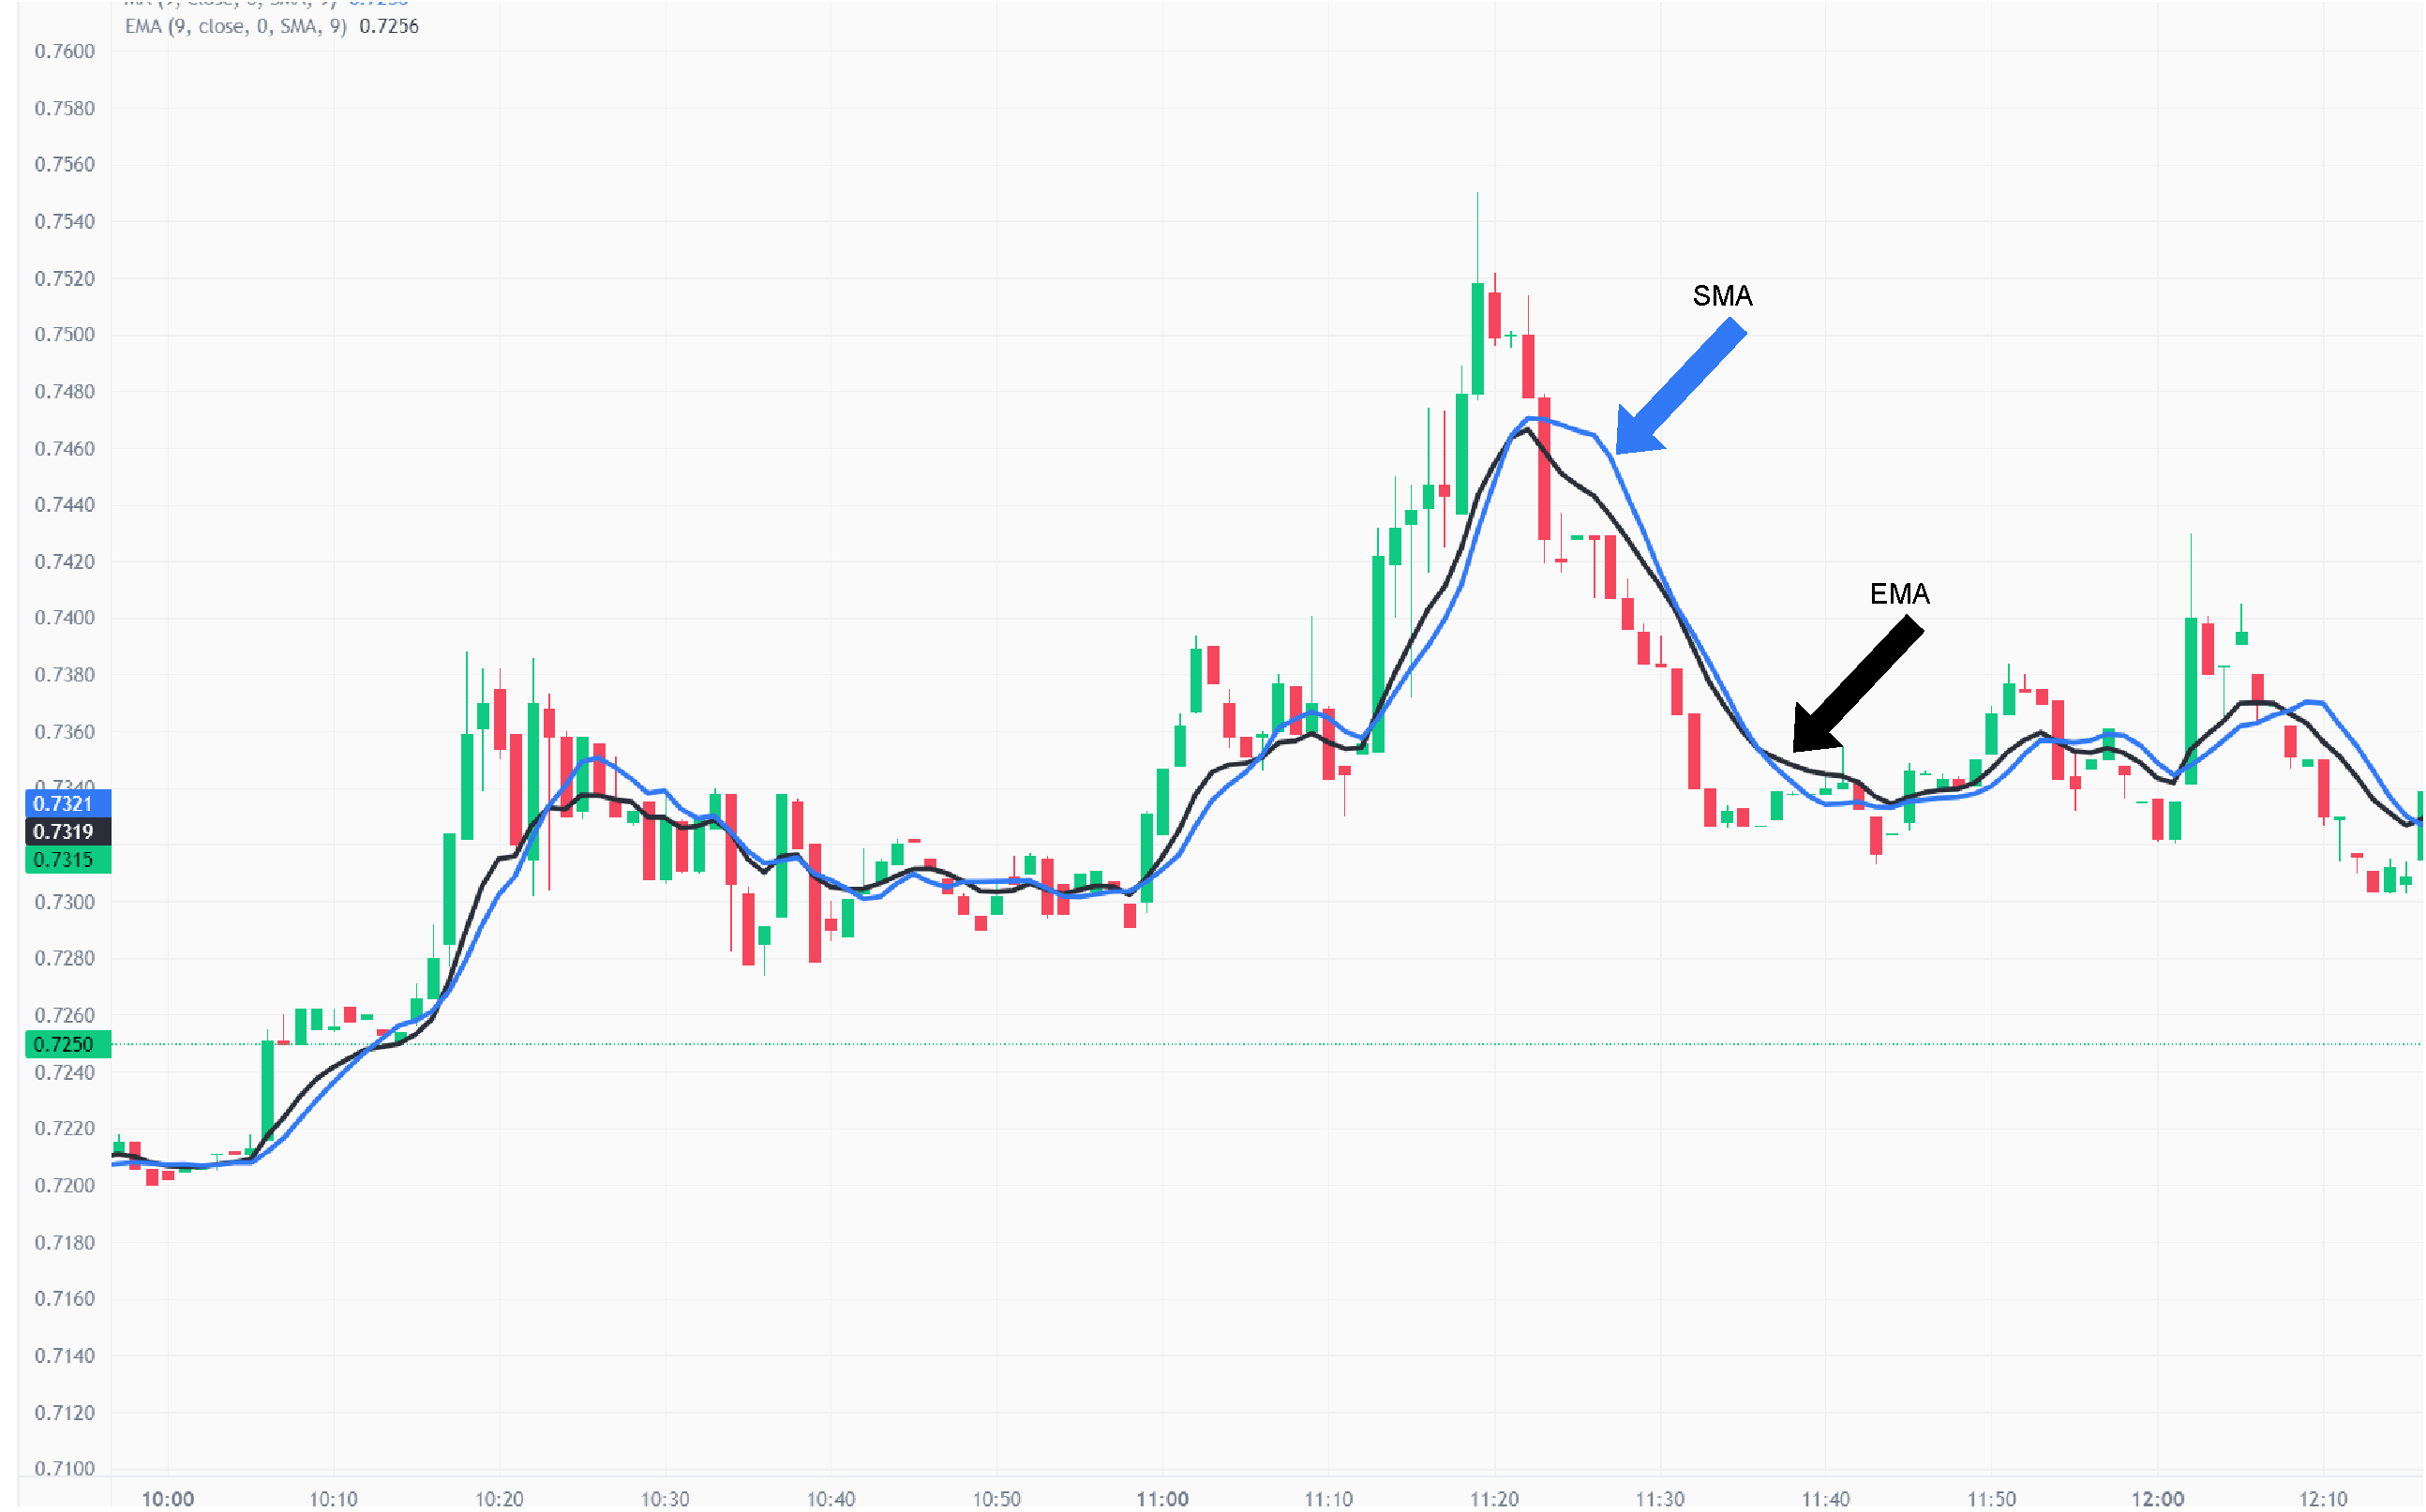
\includegraphics[width=1\textwidth]{Figures/MA.pdf}
    \caption{Znázornění indikátoru SMA a EMA \cite{tradingview}}
    \label{fig:ma-sma-ema}
\end{figure}

\subsection{Index relativní síly (RSI, Relative strength index)}
Index relativní síly patří mezi oscilující indikátory, pohybující se v rozmezí od 0 do 100. Jeho cílem je odhalit rychlost a velikost změny \enquote{close} cen aktiv a tím identifikovat
přeprodaný nebo překoupený trh. Důležité signály nastávají v momentě, kdy se hodnota tohoto indikátoru zvedne nad hladinu 70 nebo klesne pod hladinu 30 a interpretace je následující:
\begin{itemize}
    \item Pokud hodnota $RSI > 70$ je trh překoupený a má vyšší hodnotu, než by měl mít; následuje korekce nebo otočení trendu.
    \item Pokud hodnota $RSI < 30$ je trh přeprodaný a má nižší hodnotu, než by měl mít; následuje korekce nebo otočení trendu.
    \item Při opětovném sestupu pod hranici 70 je identifikován sestupný sentiment.
    \item Při opětovném vzestupu nad hranici 30 je identifikován vzestupný sentiment.
\end{itemize}
Tyto situace lze vidět i na obrázku \ref{fig:rsi}.

\begin{figure}[h]
    \centering
    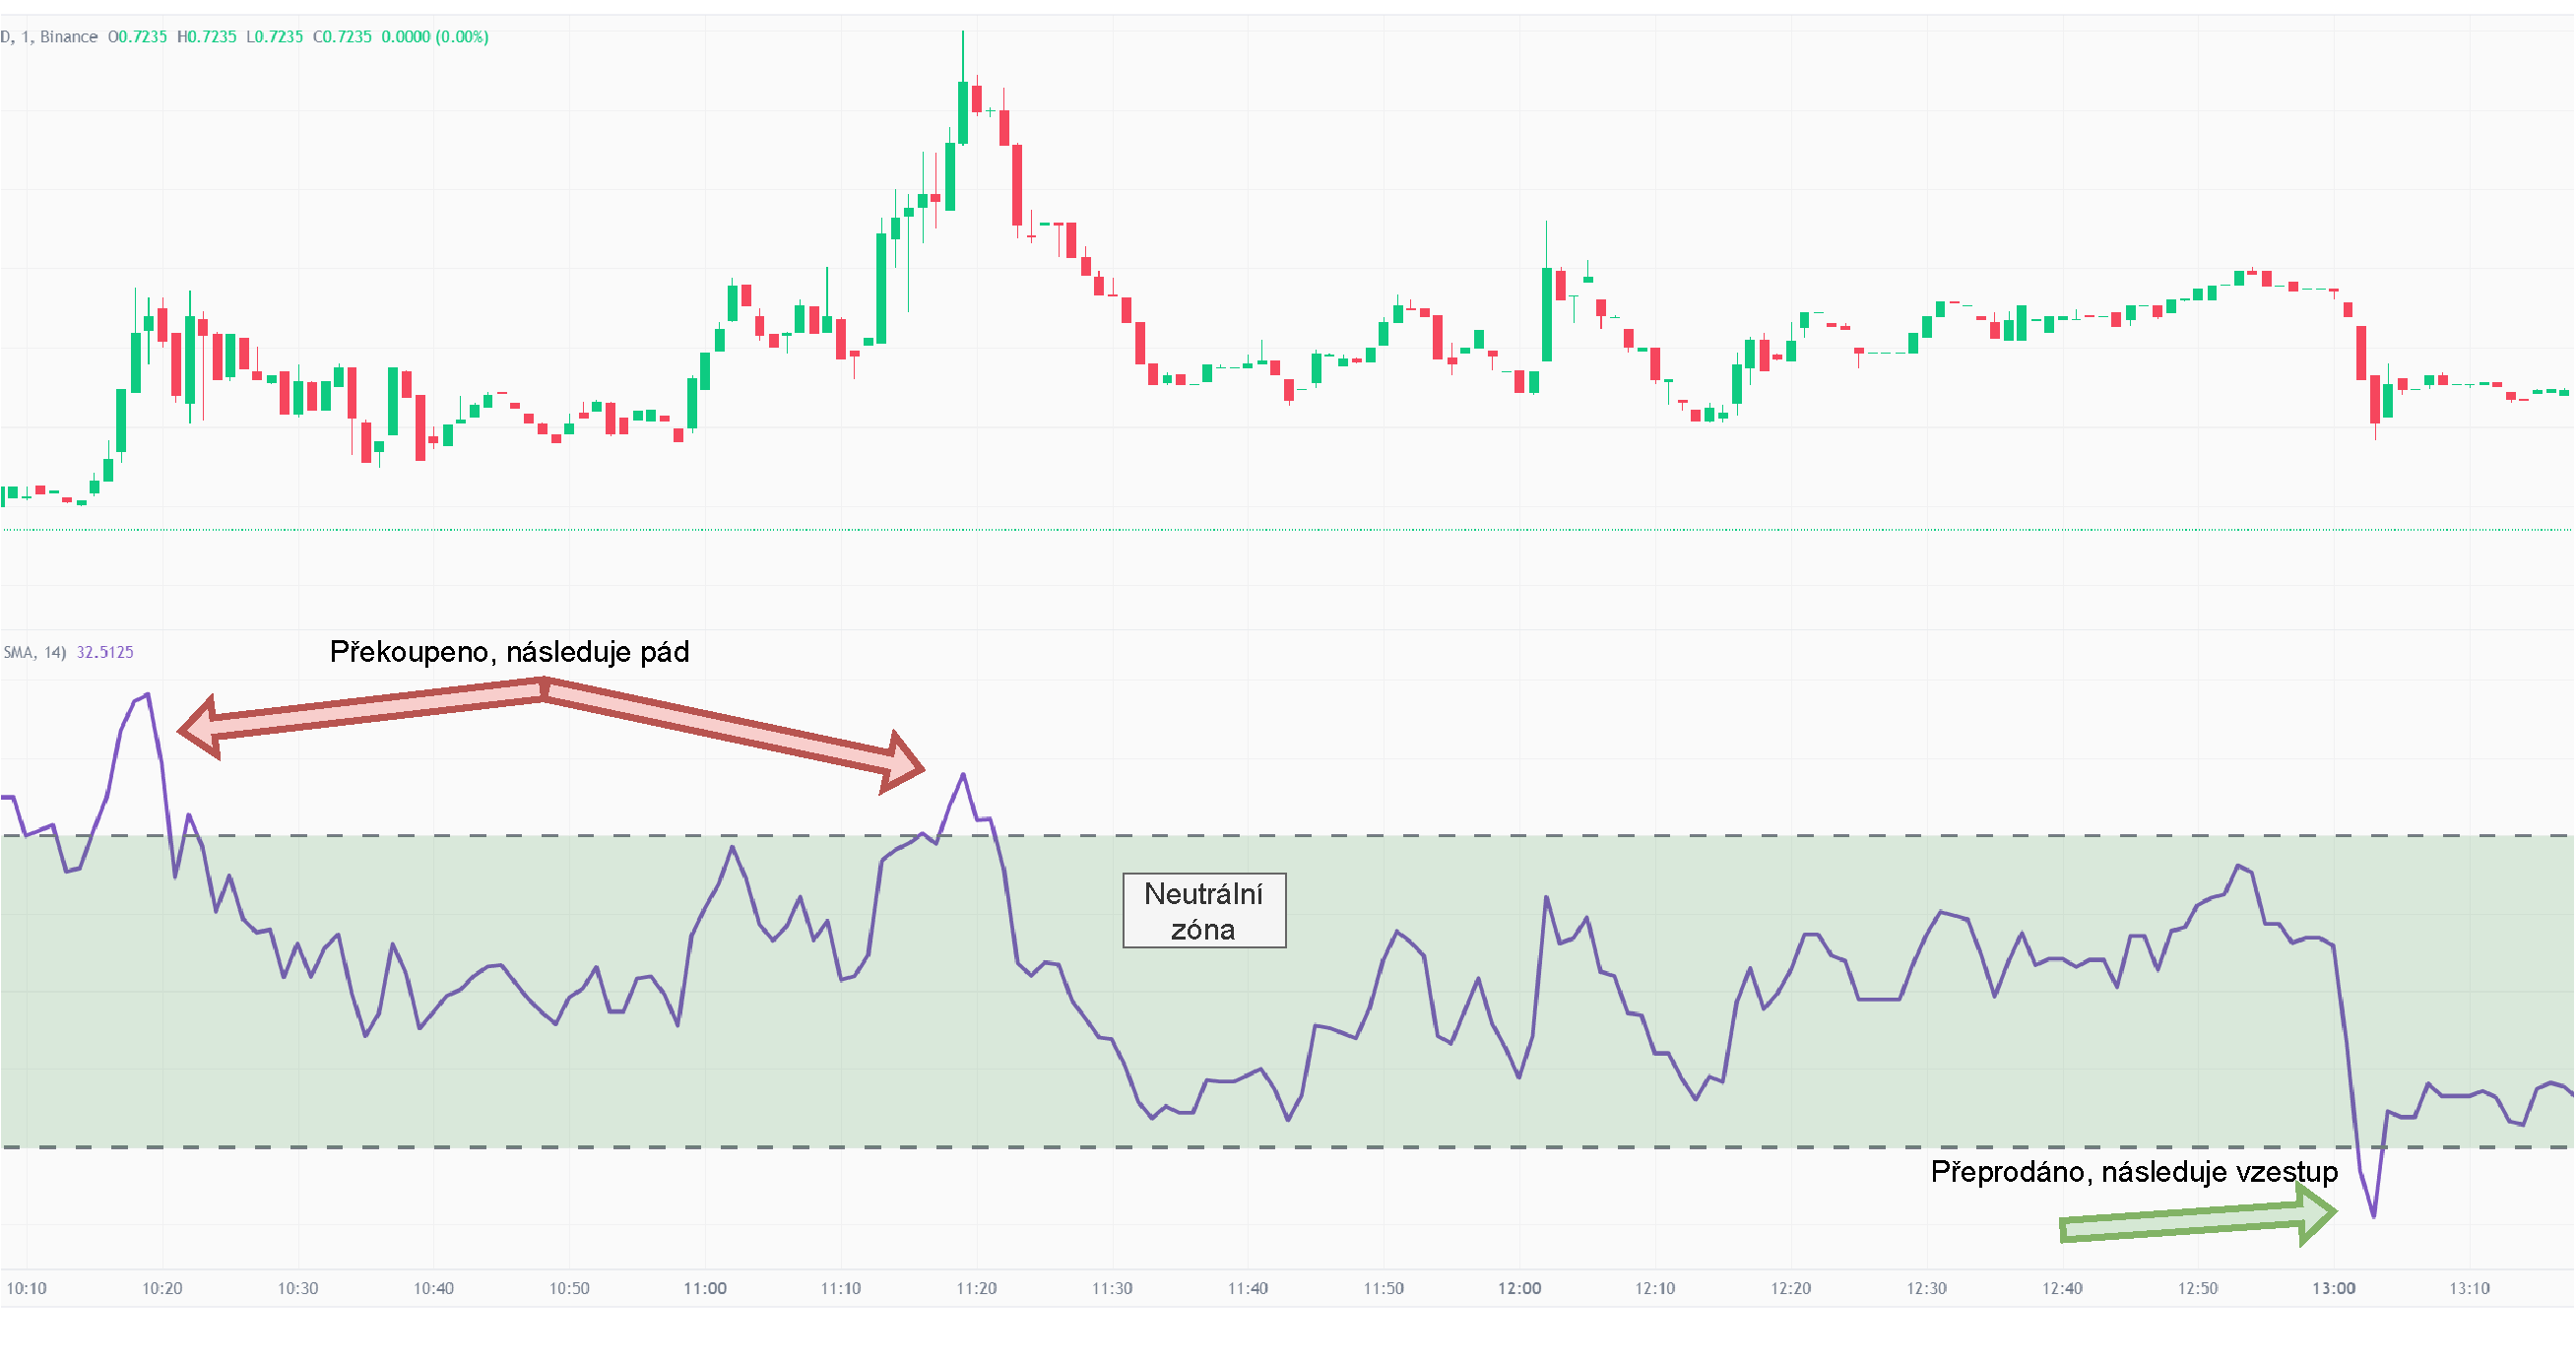
\includegraphics[width=1\textwidth]{Figures/RSI.pdf}
    \caption{Indikátoru RSI se signály překoupeného a přeprodaného trhu \cite{tradingview}}
    \label{fig:rsi}
\end{figure}

Pro výpočet indexu relativní síly je nutné nejdříve spočítat relativní sílu. Pro zjištění relativní síly, se musí nejdříve zjistit horní (\emph{U}) a dolní (\emph{D}) změna:
\begin{equation}
    U = \begin{cases}
        C_t - C_{t - 1}, & C_t > C_{t - 1}   \\
        0,               & C_t \le C_{t - 1} \\
    \end{cases}
    ,
    D = \begin{cases}
        C_{t - 1} - C_t, & C_t < C_{t - 1}   \\
        0,               & C_t \ge C_{t - 1} \\
    \end{cases}
    \label{eq:du}
\end{equation}
Pak můžeme vypočíst relativní sílu \emph{RS} za období délky \emph{n}:
\begin{equation}
    RS =
    \begin{cases}
        \frac{EMA(U, n)}{EMA(D, n)}, & {EMA(D, n)} > 0 \\
        100,                         & {EMA(D, n)} = 0
    \end{cases}
    \label{eq:rs}
\end{equation}
A nakonec dopočítat index:
\begin{equation}
    RSI = 100 - \frac{100}{1 + RS}
    \label{eq:rsi}
\end{equation}

\subsection{MACD indikátor (Moving average convergence-divergence indicator)}
Indikátor sbíhavosti a rozbíhavosti klouzavých průměrů se skládá z několika komponent. První je samotný MACD (vzorec \ref{eq:macd}), což je rozdíl dvou exponenciálních klouzavých průměrů, počítané
za kratší a delší období. Další složkou je signální čára (vzorec \ref{eq:signal}), vypočítaná jako EMA právě onoho MACD. Poslední složka je histogram (vzorec \ref{eq:macdhist})
ukazující rozdíl mezi MACD a signální čárou. Vizualizace tohoto indikátoru je vidět na obrázku \ref{fig:macd}

\begin{equation}
    MACD = EMA(n_1) - EMA(n_2), n_2 > n_1
    \label{eq:macd}
\end{equation}

\begin{equation}
    Sig_{MACD} = EMA(MACD, n_3)
    \label{eq:signal}
\end{equation}

\begin{equation}
    Hist_{MACD} = MACD - Sig_{MACD}
    \label{eq:macdhist}
\end{equation}

Signál pro nákup nebo prodej aktiva nastává v momentě, kdy MACD protne signální čáru. Pro zachycení vzestupného trendu musí MACD protnout signální čáru zespodu. Pro zachycení
trendu sestupného je situace opačná, kdy MACD musí protnout signální čáru shora. % TODO: Dodelat obrazky

\begin{figure}[h]
    \centering
    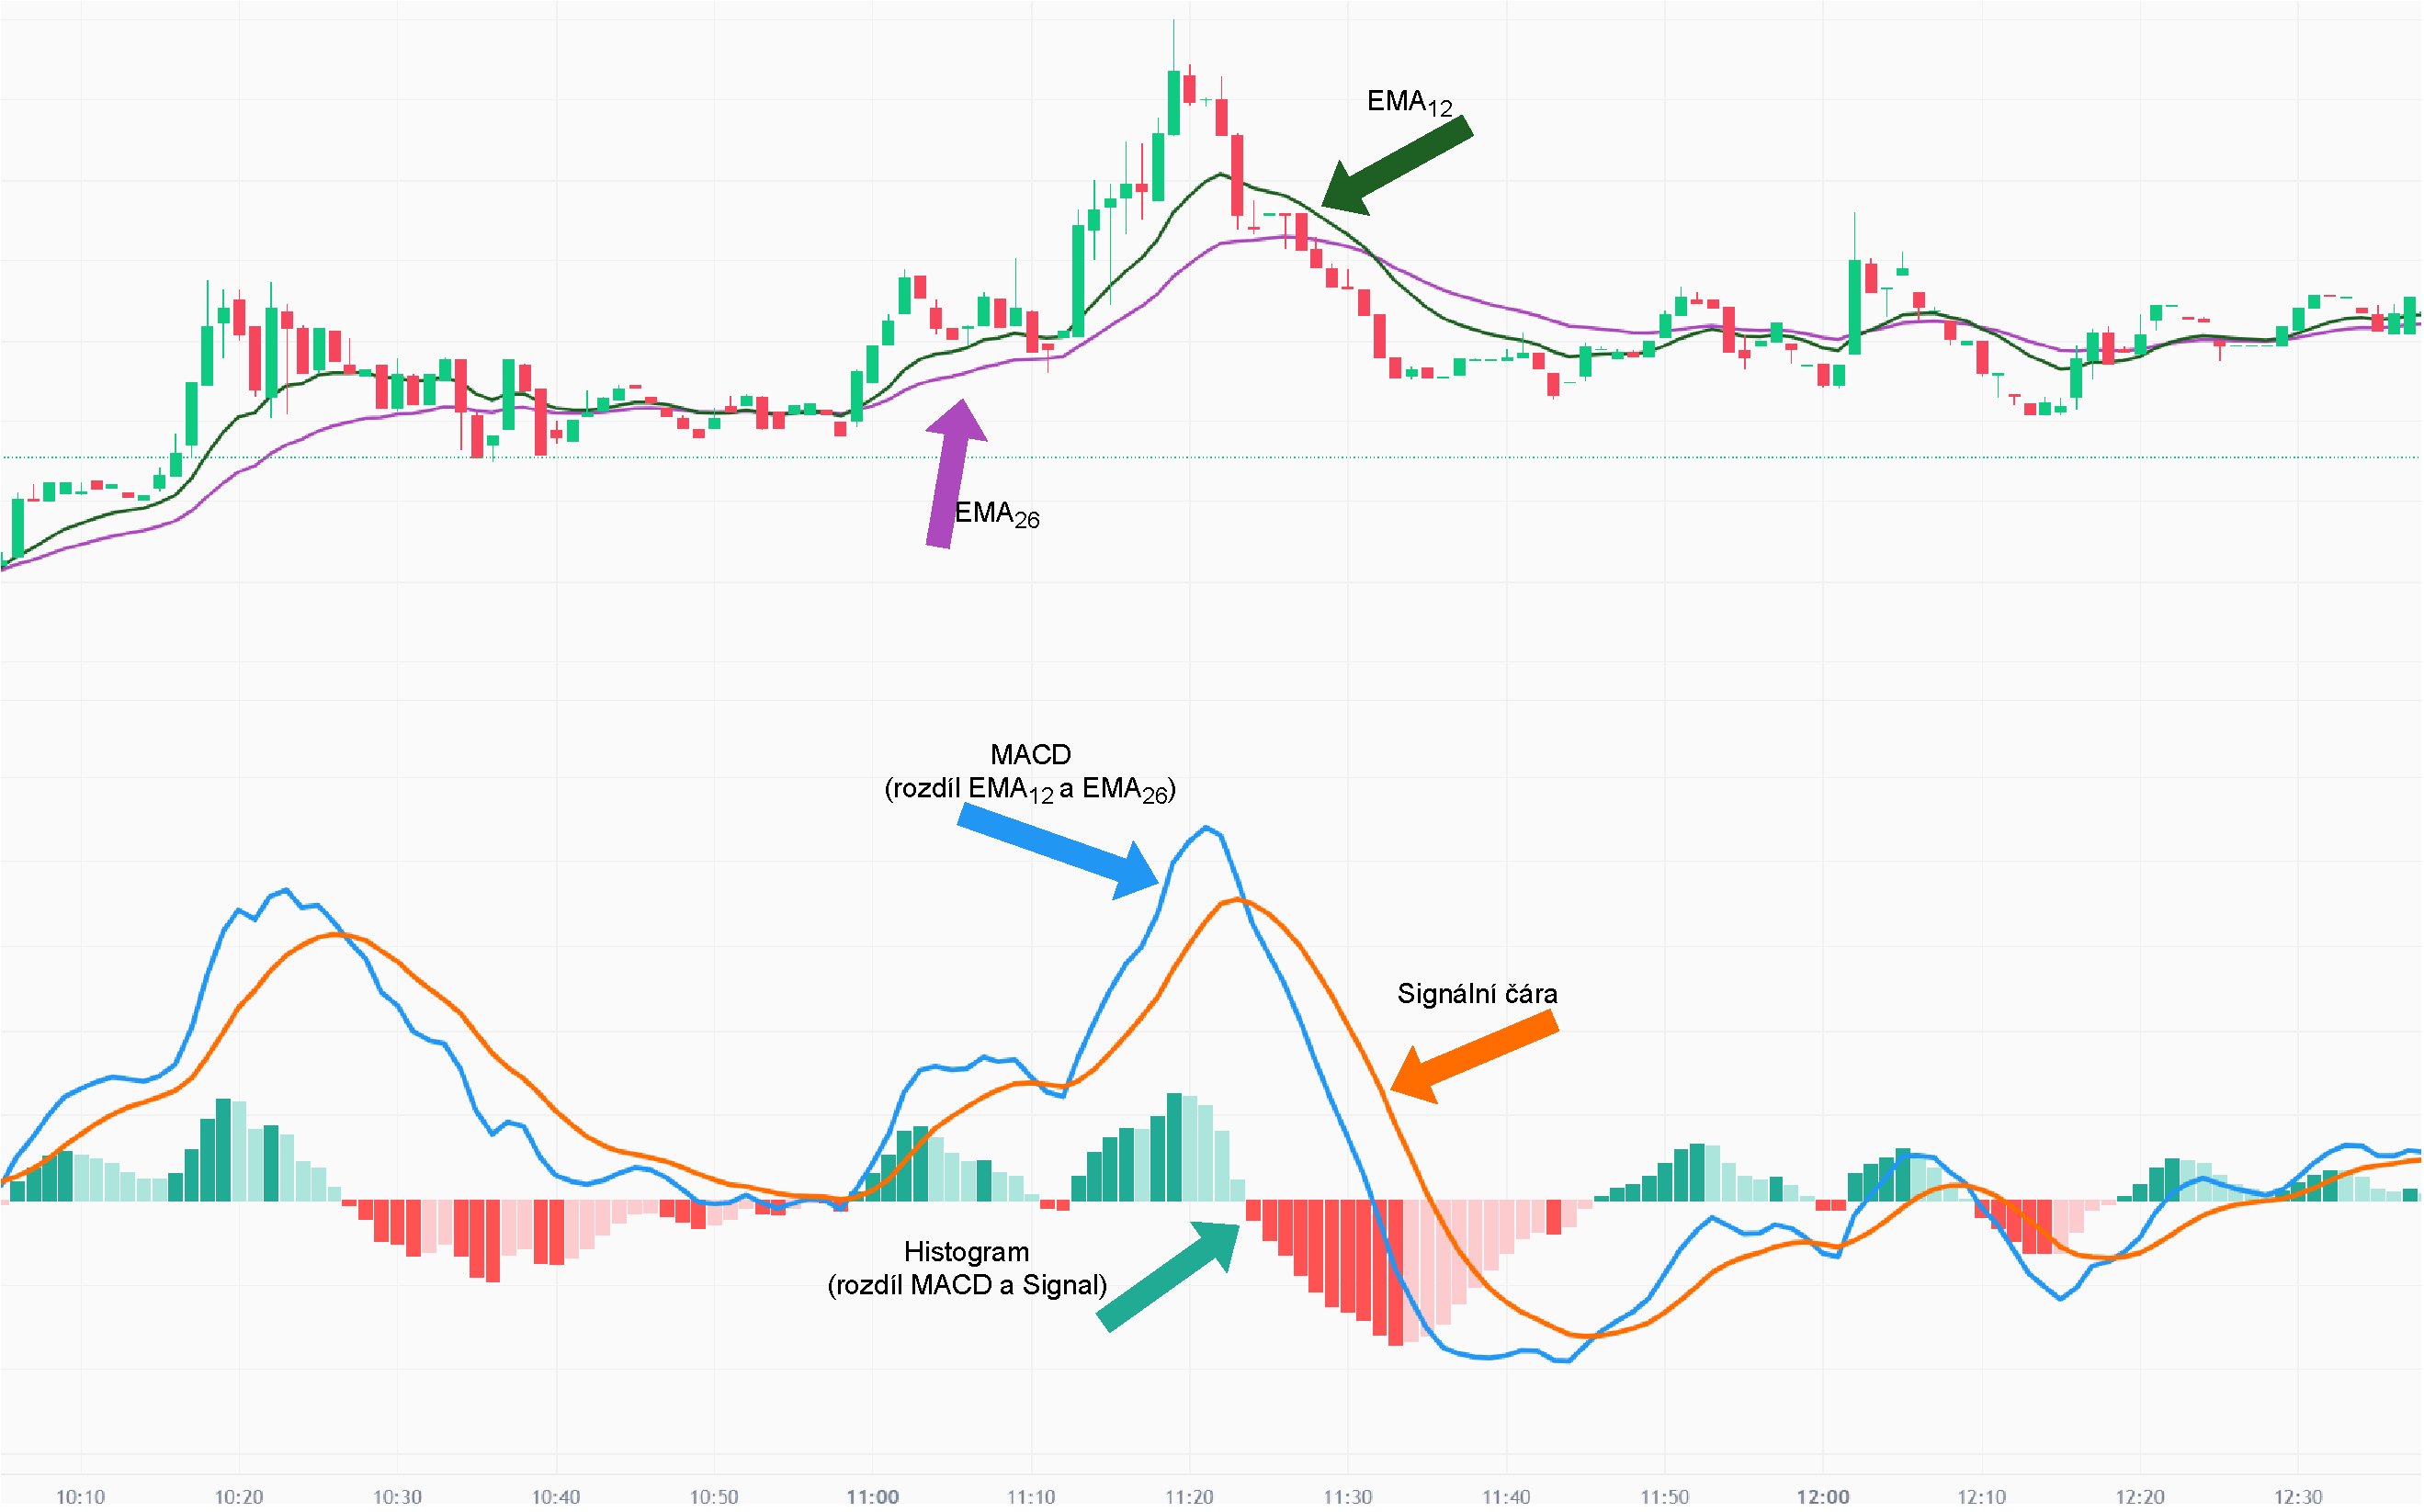
\includegraphics[width=1\textwidth]{Figures/MACD.pdf}
    \caption{Znázornění indikátoru MACD s popisem \cite{tradingview}}
    \label{fig:macd}
\end{figure}

\subsection{Stochastický oscilátor}
Další ze skupiny oscilátorů je hojně využívaný stochastický oscilátor, rovněž určený k zachycení rychlosti změny ceny a identifikace překoupeného nebo přeprodaného trhu. Jeho
hodnoty se typicky pohybují v rozmezí 0 až 100 (případně 0 až 1). Myšlena tohoto oscilátoru spočívá v úvaze, že ceny, před obratem trendu, mají tendenci se uzavírat blízko extrémů
nedávných obchodů. Jako klíčové hodnoty pro označení překoupeného respektive přeprodaného trhu se považují 80 a 20. Souběžně s tímto oscilátorem se využívá vyhlazovací
klouzavý průměr periody o velikosti 3. Pro výpočet hodnot stochastický oscilátoru se používá vzorec \ref{eq:sto}, kde $L_{obd}$ a $H_{obd}$ značí nejnižší a nejvyšší cenu za specifikované
období.

\begin{equation}
    STO = 100 * \frac{C  - L_{obd}}{H_{obd} - L_{obd}}
    \label{eq:sto}
\end{equation}


\begin{figure}[ht]
    \centering
    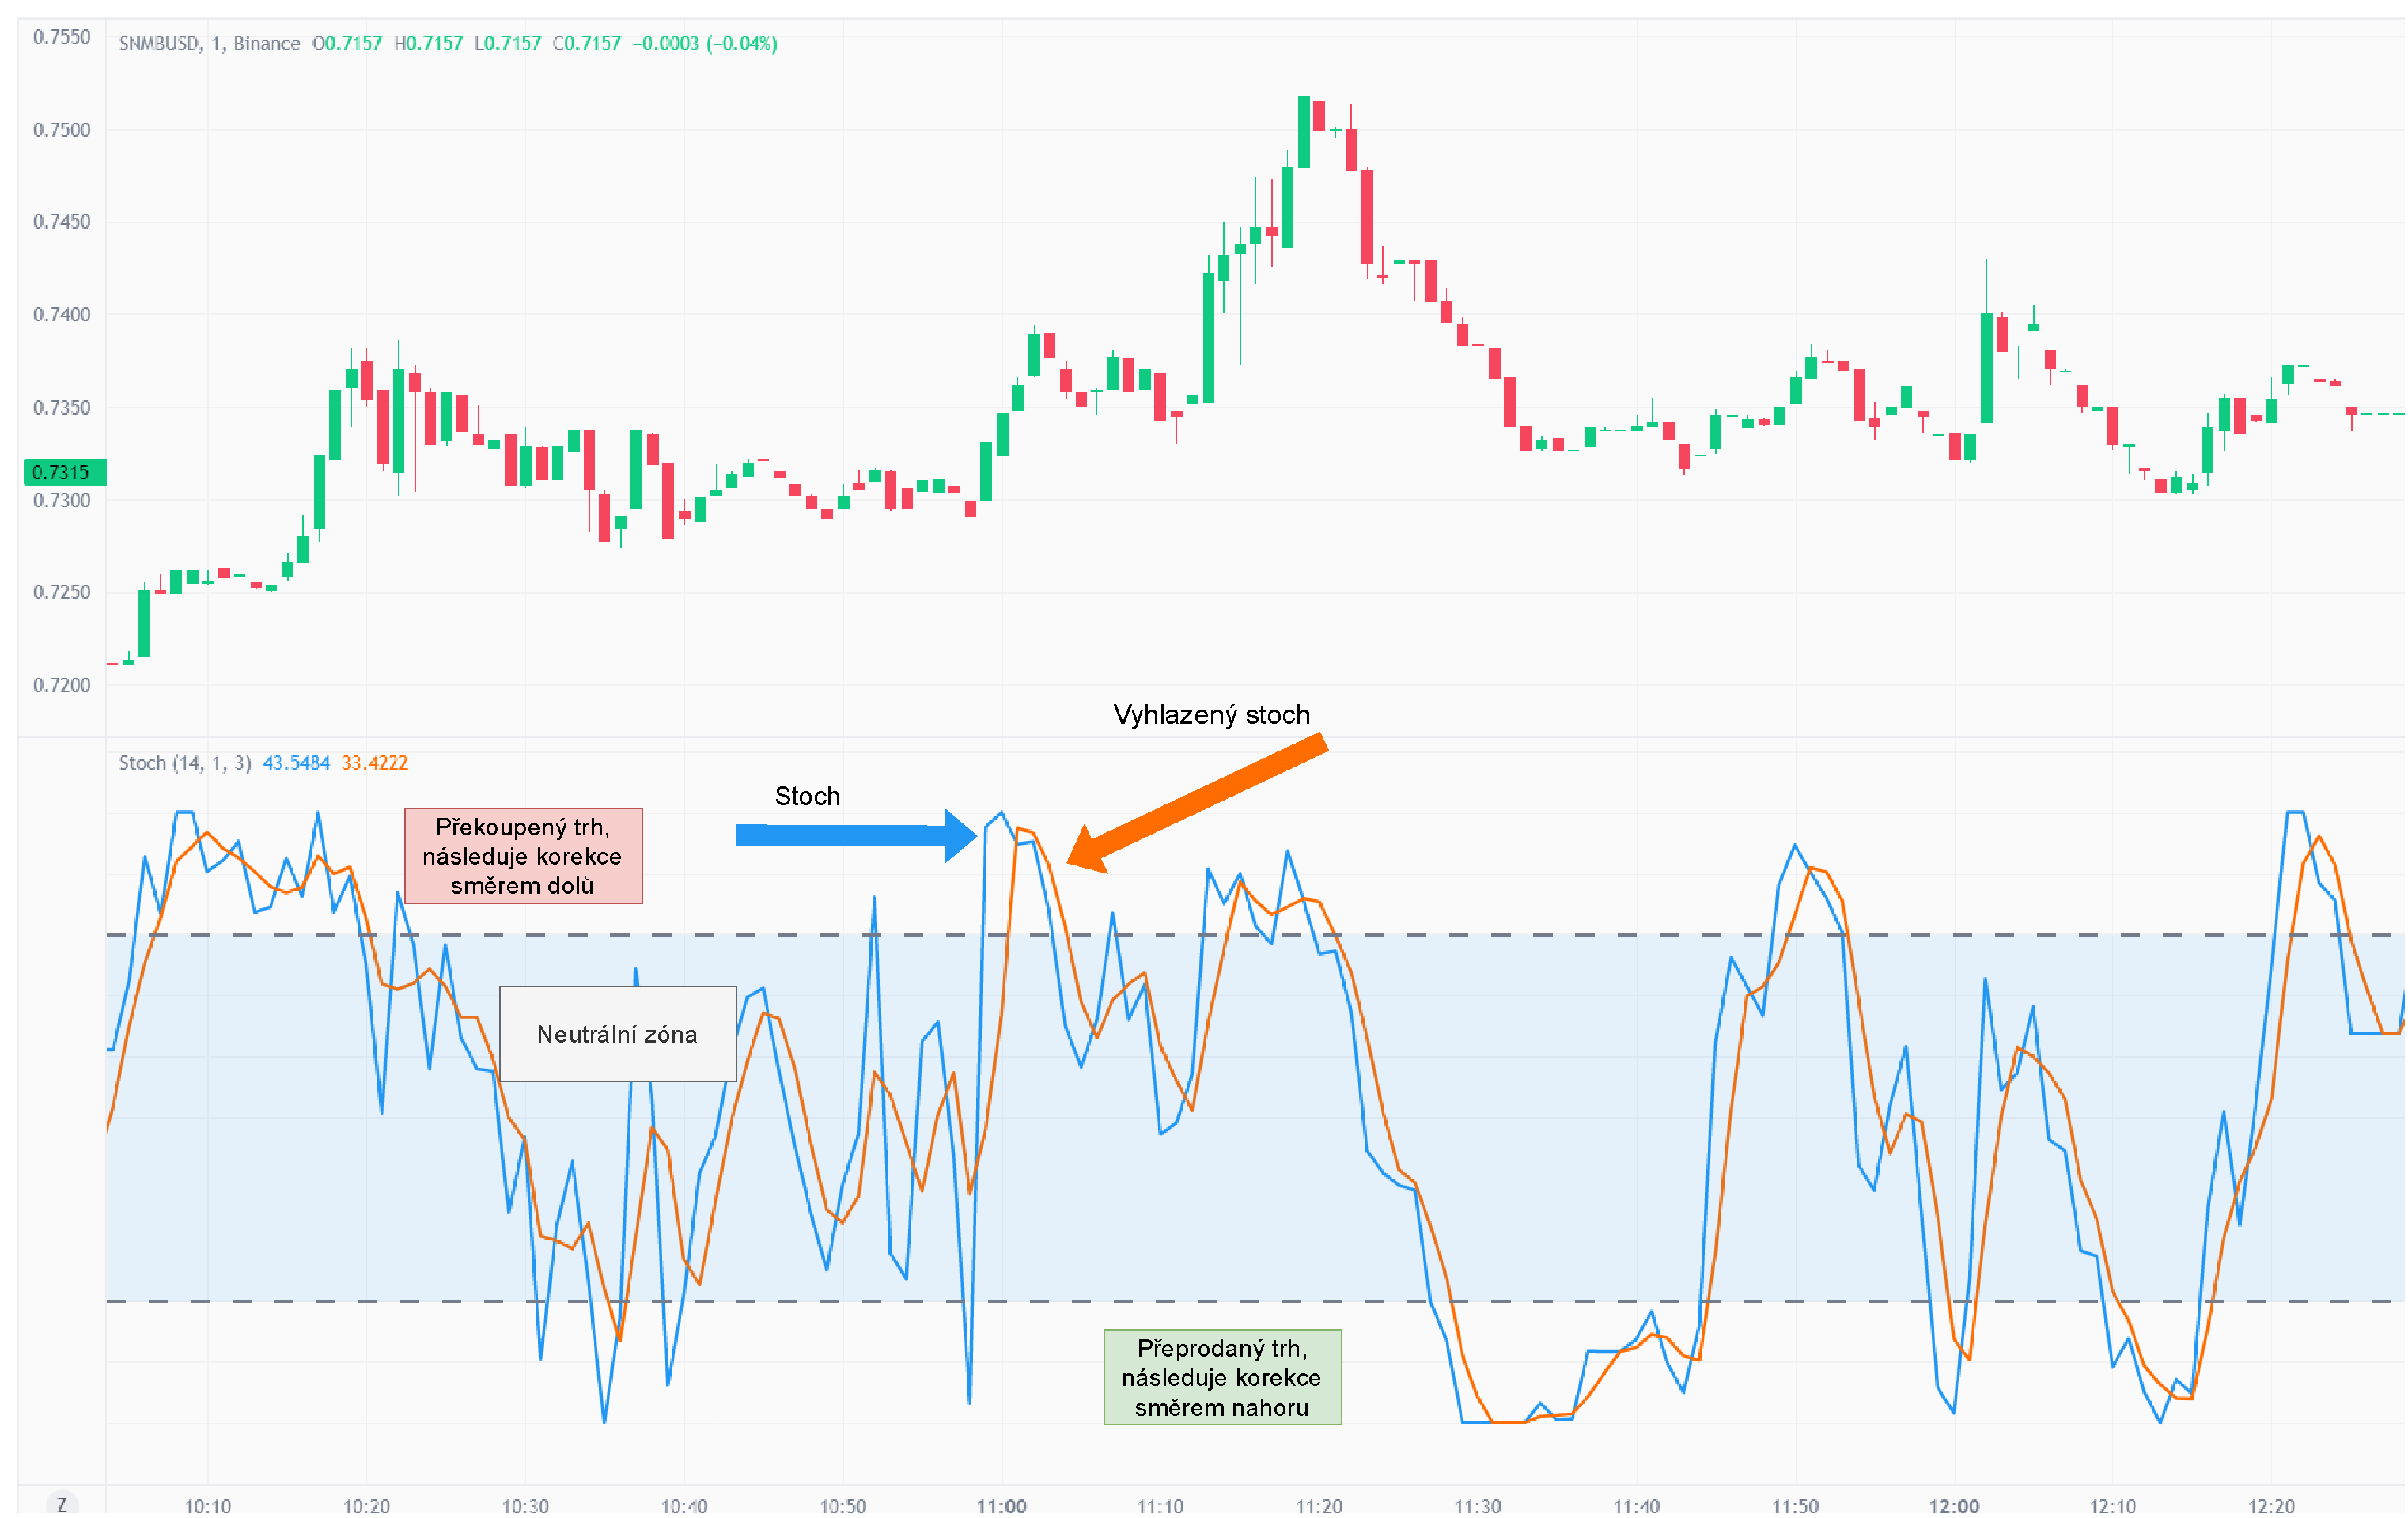
\includegraphics[width=0.8\textwidth]{Figures/Stoch.pdf}
    \caption{Stochastický oscilátor \cite{tradingview}}
    \label{fig:stoch}
\end{figure}

\subsection{Bollingerova pásma (BB, Bollinger Bands)}
Poslední z indikátorů jsou Bollingerova pásma, měřící volatilitu trhu. Skládá se celkem ze 3 pásem - horní, střední a spodní pásmo. Tato pásma nejsou nic jiného než klouzavé průměry
s drobnou změnou. Jako klouzavý průměr se nejčastěji využitá jednoduchý SMA, ale lze využít i jakýkoli jiný typ, například EMA. Horní a spodní pásmo se získá připočtením a odečtením
(obvykle 2) násobku standardní odchylky $\sigma$ (vzorec \ref{eq:bb}). Se snižující nebo zvyšující se volatilitou dochází k tzv. kontrakci nebo roztažení pásem (viditelné na obrázku \ref{fig:bb}).
Pokud je volatilita nízká, budou mít
pásma tendenci přibližovat se k sobě a dochází ke kontrakci. Opačným případem je roztažení. Signál překoupení aktiva nastává, pokud se tržní cena přiblíží hornímu pásmu. Naopak přeprodání
nastane, pokud se cena nachází v blízkosti spodního pásma. Může dojít i k proražení těchto pásem, což může naznačovat extrémní tržní podmínky.

\begin{equation}
    Band_{up + down} = MA \pm K\sigma
    \label{eq:bb}
\end{equation}

\begin{figure}[ht]
    \centering
    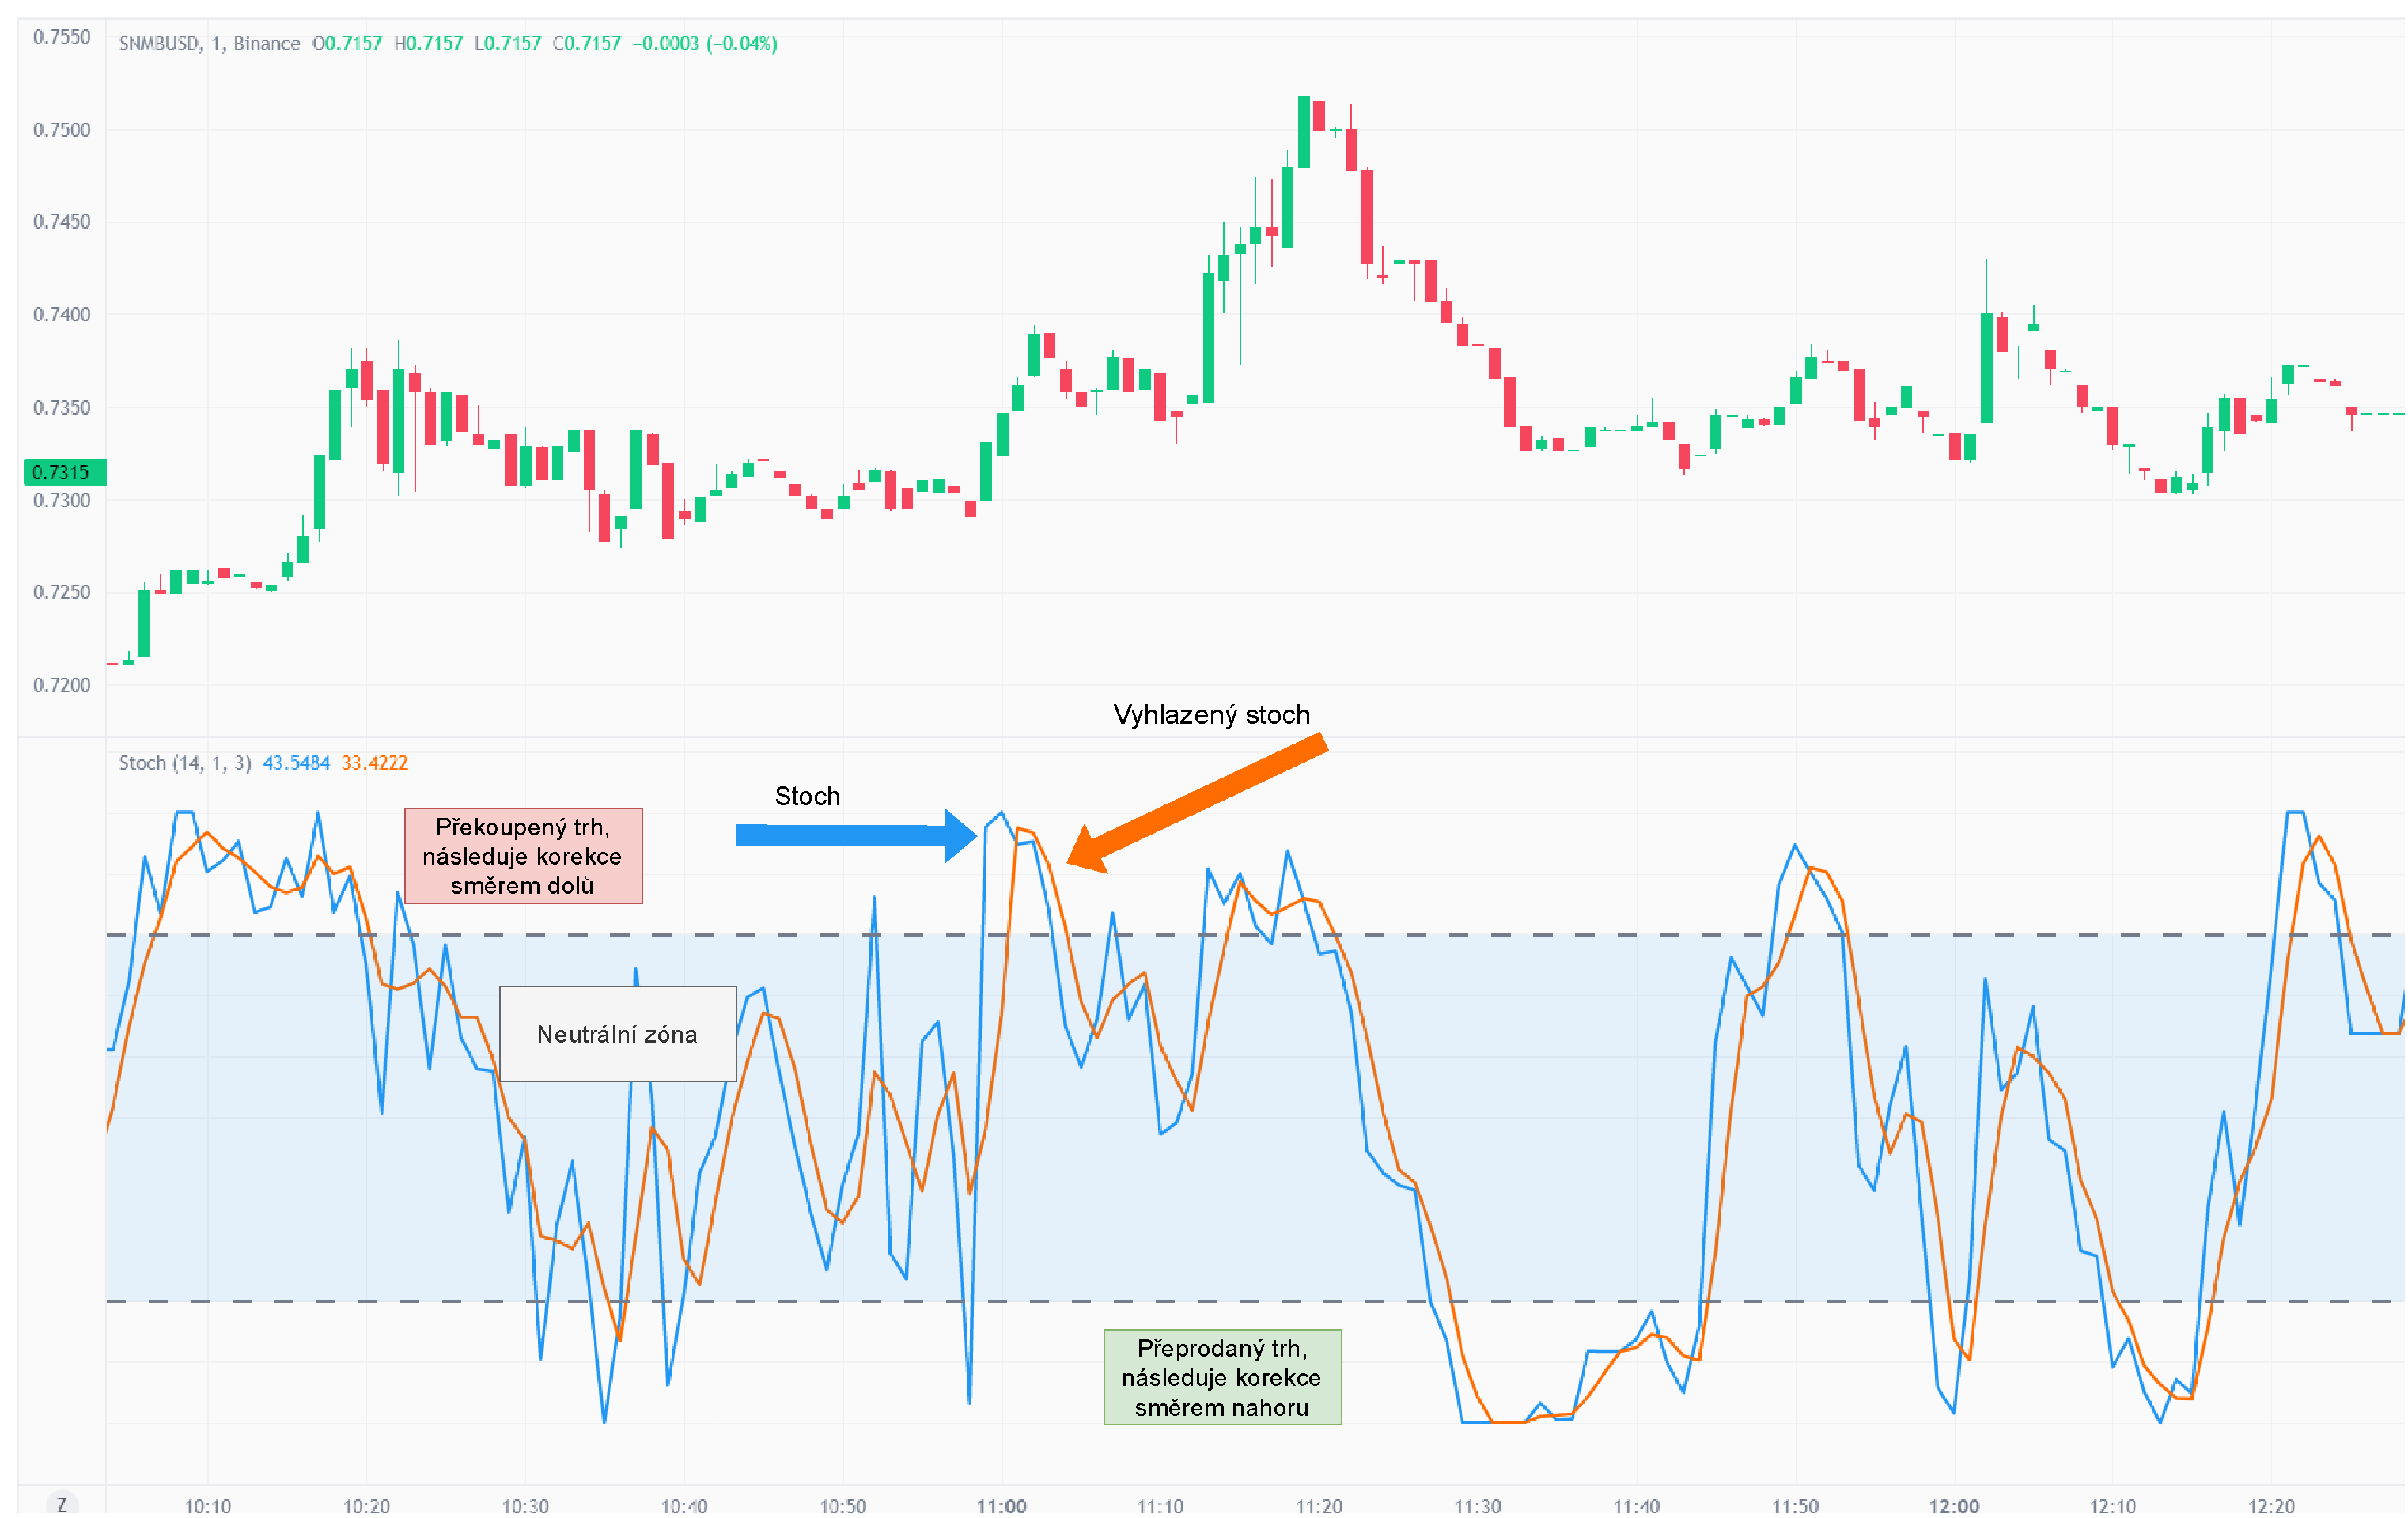
\includegraphics[width=0.8\textwidth]{Figures/Stoch.pdf}
    \caption{Bollingerova pásma s vizualizací kontrakce a roztažení \cite{tradingview}}
    \label{fig:bb}
\end{figure}


\endinput